\documentclass[11pt]{article}
\usepackage{geometry}
\geometry{letterpaper}

\usepackage{amssymb,amsmath} %Standard libraries that add lots of equation features and math symbols
\numberwithin{equation}{subsection} %This makes equations numbered by section rather than sequentially overall. 
\usepackage[labelsep=period]{caption}
\usepackage{subcaption}
\usepackage{hyperref} %Adds some useful tricks with references
\hypersetup{ %Makes all sections in ToC, figure and table numbers, and references clickable
    colorlinks=false, %set true if you want colored links
    linktoc=all,     %set to all if you want both sections and subsections linked
}
\usepackage{setspace}
\usepackage{fullpage}
\usepackage{titlesec}
\usepackage{paralist,multirow}
\usepackage{tikz} %Package for making diagrams
\usetikzlibrary{decorations.pathreplacing, calc} 
\usetikzlibrary{snakes,shapes,decorations.text}

\newcommand{\degrees}{\ensuremath{^\circ}} % type /degrees when in paragraph mode to insert a degree symbol
\newcommand{\sectionbreak}{\clearpage}

%=======================================%=======================================%
%\usepackage{physics}
\usepackage{soul}

% figure has no top padding
\makeatletter
\setlength{\@fptop}{0pt}
\makeatother

\definecolor{crimson}{RGB}{220, 20, 60}
\definecolor{deepskyblue}{RGB}{0, 191, 255}
\definecolor{orchid}{RGB}{186, 85, 211}
\definecolor{seagreen}{RGB}{60, 179, 113}
\newcommand{\vp}[1]{\textcolor{crimson}   { #1 }}
\newcommand{\tk}[1]{\textcolor{deepskyblue}{ #1 }}
\newcommand{\gz}[1]{\textcolor{orchid}{ #1 }}
\newcommand{\nb}[1]{\textcolor{seagreen}{ #1 }}

\usepackage[parfill]{parskip} % defaults to \noindent and paragraph spacing of 1 line.

\newcommand{\vvis}{vis-\`a-vis}
\newcommand{\unit}[1]{\ensuremath{\, \mathrm{#1}}}             % units
\newcommand{\eqn}[1]{\begin{equation}\begin{split}#1\end{split}\end{equation}}
\newcommand{\nvect}[1]{\underline{#1}}                         % vector associated with discretization
\newcommand{\vect}[1]{\boldsymbol{#1}}                         % vector field
\newcommand{\uvect}[1]{\boldsymbol{\hat{#1}}}                  % unit vector
\newcommand{\tensor}[1]{\underline{\underline{#1}}}            % second order tensor field
\newcommand{\der}{\,\mathrm{d}}                                % dx ==> \der x
\newcommand{\Der}{\,\mathrm{D}}                                % Du ==> \Der u
\newcommand{\del}{\vect{\nabla}}                               % gradient vector operator
\newcommand{\grad}{\del}                                       % gradient vector operator
\newcommand{\ppp}[1]{\partial_{#1}}                            % partial derivative
\newcommand{\ddd}[1]{\dfrac{\mathrm{d}}{\mathrm{d} #1}}        % total derivative
\newcommand{\material}{\mathrm{D}_{t}}                         % material derivative (wrt time)
\newcommand{\defeq}{\mathrel{\mathop:}=}                       % define equal to
\newcommand{\degree}{^\circ}                                   % degree
\newcommand{\component}[1]{\langle #1 \rangle}                 % vector components (also scalar product too)
\newcommand{\vvec}[1]{\begin{pmatrix}#1\end{pmatrix}}          % vector components (# \\ #)
\newcommand{\mat}[1]{\begin{bmatrix}#1\end{bmatrix}}           % matrix
\newcommand{\transp}{\intercal}                                % matrix transpose A^\transp
\newcommand{\expo}[1]{\mathrm{e}^{#1}}                         % e = 2.71..
\newcommand{\al}{\alpha}                                       % \alpha
\newcommand{\supp}[1]{\mathrm{supp}(#1)}                       % support of a function
\newcommand{\subsubset}{\subset\subset}                        % A\subsubset B iff closure of A compact subset of B
%=======================================%=======================================%

\begin{document}

\begin{titlepage}
\newcommand{\HRule}{\rule{\linewidth}{0.5mm}}
\center
\textsc{\LARGE University of Illinois at Urbana-Champiagn}\\[1cm]
\textsc{\Large ME 470: Senior Design}\\[1cm]
\HRule \\[0.4cm]

{ 
  \huge \bfseries Battery Cooling for Illini Hyperloop \\[0.5cm]
  \large Final Report\\[0.5cm]
}

\HRule \\[1cm]
{\Large \today}\\[1cm]
\emph{Authors:}\\
\begin{tabular}{l r l}
  Vedant Puri        & \texttt{vpuri3@illinois.edu}  &  (347)-330-1343 \\
  Nabarun Banerjee   & \texttt{nkb2@illinois.edu}    &  (217)-979-3559 \\
  Tanner Koehne      & \texttt{koehne2@illinois.edu} &  (217)-313-1351 \\
  Gordon Zak         & \texttt{gzak2@illinois.edu}   &  (321)-645-7910 \\
\end{tabular}\\[0.5cm]
\emph{Advisor:} \\
Dr. Blake Johnson\\[0.5cm]
\emph{Teaching Assistant:} \\
Hae Woo Chung \\[0.5cm]
\emph{Submitted To:} \\
Dr. L Winston Zhang \\
Novark Technologies, Inc.\\
Boanan Road \#63\\
Longgang Nanlian Industry Zone \#6\\
Shenzhen, Guangdong, China 518116\\[0.5cm]
\vfill

\end{titlepage}

\tableofcontents
\listoffigures
\begingroup
\let\clearpage\relax
\listoftables
\endgroup

%\newpage
%{\huge
%\vp{Vedant}\vspace{1em}
%\tk{Tanner}\vspace{1em}
%\gz{Gordon}\vspace{1em}
%\nb{Nobby}}
\newpage
%========================================================================
\onehalfspacing

\section{Executive Summary}
Illini Hyperloop RSO, a constituent member of the Midwest Hyperloop team, is competing in the fourth SpaceX Pod Competition, where teams design and build pods to race at high speed down a 1250 meter long evacuated tube. The team's hyperloop pod will be propelled by an electric motor powered by a $111\unit{V}$ Lithium-Polymer (Li-Po) battery pack, passing current of up to $800\unit{A}.$ Upper estimates reveal that the total heat loss incurred in the battery pack is $300\unit{kJ}.$ The senior design team developed a battery cooling system for the pod, as heat generated in the discharge of Li-Po batteries can negatively effect performance and pose safety hazards. SpaceX regulations demand that the hyperloop pod batteries not exceed $50\degree\unit{C}$ in temperature.

The senior design team modelled the pod's propulsion system---battery pack, motor controller and motor---to estimate power requirements and heat losses. A key assumption made was that battery performance is temperature invariant. As battery components heat up unevenly during discharge, the team performed qualitative tests on a single Li-Po battery to locate regions susceptible to overheating by studying trends in heat generation in batteries under operation. The team identified patterns in regions of heat concentrations and focused cooling efforts in those areas.

The delivered battery cooling solution effectively removes heat dissipated by the battery over a twenty-second competition run. The cooling solution consists of hollow aluminium brazed plates filled with water. The brazed plates have fins in the interior to improve heat transfer from aluminium to water. The team performed finite element analysis to verify that the cooling system can absorb the energy produced without exceeding $50\degree\unit{C}$, starting with an ambient temperature of $30\degree\unit{C}.$

As Li-Po pouch batteries are not rated to operate in vacuum, the senior design team assisted Midwest Hyperloop in designing a pressure vessel maintained at $1\unit{atm}$ to house the battery packs, cooling solution, and electronic controllers. The battery box is constrained in length and height by the pod chassis and aerodynamic constraints.

The team considered relevant environmental and social impacts, referenced appropriate standards, and completed the project under budget. Plate shipping and battery procurement were the primary expenses. The brazed plates required for the passive cooling system were manufactured by the senior design project sponsor, Novark Technologies.

\pagebreak 
%========================================================================
\section{Introduction and Problem Statement}
Hyperloop is a proposed mode of transportation where pods carrying passengers or freight travel at high speeds in an evacuated tube. The lack of air resistance makes travel in hyperloop efficient. Initial designs released by Tesla and SpaceX showed a pod that would be accelerated to cruising speed with the help of linear electric motors and glide on air bearings above their track through tubes. Current prototypes of the hyperloop developed by other independent operators also use magnetic levitation and hybrid systems with high speed wheels to eliminate friction with the track.

\subsection{Hyperloop Pod Competition}
The hyperloop pod competition is sponsored by SpaceX. Participating teams build a sub-scale prototype to demonstrate the feasibility of their design. The competition is held annually in August in Hawthorne, CA. The competition has three phases: design, fabrication, and the race. A panel of SpaceX engineers scrutinise the safety aspects of the prototype before the team is allowed to advance to the next round. The race is over a distance of 1.51\unit{km} which Midwest Hyperloop plans to complete in 20 seconds.

Illini Hyperloop is competing in the fourth SpaceX Hyperloop Pod competition. Illini Hyperloop is collaborating with hyperloop teams from Purdue University and University of Cincinnati to form the consortium Midwest Hyperloop. Illini Hyperloop will manage the propulsion system for the Midwest Hyperloop pod.

\subsection{Pod Overview}
The Midwest Hyperloop pod will be about 6.5 feet long, have a mass of around 135 kg, and will be propelled by an EMRAX 228 Low-Voltage motor. The EMRAX 228 is a permanent magnet synchronous motor modulated by an EMSISO EmDrive 500 motor controller.

Figure \ref{fig:pod} illustrates the proposed design of the 2019 pod. The aerodynamic shell located in the front of the pod will be manufactured using low density foam and layers of $3\unit{K}$ carbon fiber. The hydraulic systems and pneumatic system are enclosed by the chassis and at the rear of the chassis respectively. The motor, belt tensioner, and main drive wheel are located under the front shell. The large cylinder mounted to the middle of the chassis is the pressurised battery box designed by the senior design team. The box is positioned in the centre of the chassis as it is the heaviest component of the pod at about $32\unit{kg}$.

\begin{figure}[!htb]
 \centering
	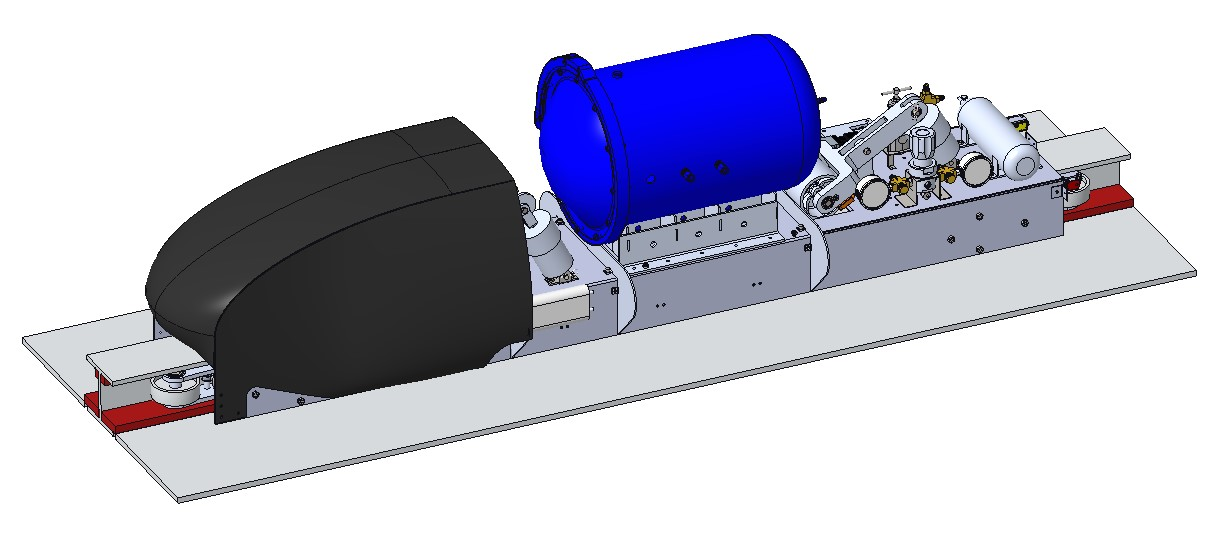
\includegraphics[width=1.0\textwidth]{final/fig/pod.jpg}
    \caption{Midwest Hyperloop Pod}
    \label{fig:pod}
\end{figure}

\subsection{Problem Statement}
There are several challenges involved in designing a hyperloop pod. The high electrical currents required to propel the pod to a speed of $100\unit{m/s}$ pose safety risks and require special equipment and handling. As power losses increase with the square of the current, passing large currents, even through small resistances, would produce heat that may damage the battery. SpaceX requires that no battery component exceed $50\unit{\degrees C}$. The objective of the senior design project is to design a cooling solution for the batteries of Midwest Hyperloop pod that meets regulations set by SpaceX, as well as the design constraints of the team.

The batteries selected by Illini Hyperloop are soft-shelled, and therefore not rated for vacuum. The current design proposes to contain the battery pack and motor controller in a pressurised battery box maintained at $1\unit{atm}$ absolute. The cooling system must fit within the space constraints of the battery box, and it must not draw power from the batteries it is supposed to cool. The motor is another source of major heat generation and is rated for a maximum temperature of $100\degree\unit{C}$. Heat dissipation is a major challenge as the pod itself is in a partial vacuum, eliminating the options of heat loss via convection or conduction to the environment.

\pagebreak

\subsection{Project Constraints}
The partial vacuum conditions the hyperloop pod operates within does not permit heat dissipation to the environment. Any heat produced must be stored within the pod as there are no outlets for heat discharge. The rate of heat transfer into the cooling system is another important consideration as heat needs to be absorbed from the battery within a 20 second period. Special considerations need to be made for the high currents passed during the competition run. The plastic casings of the batteries also pose a challenge as they have very low thermal conductivity and are effectively insulators between the interior of the batteries and the proposed cooling solution.

The cooling solution has been manufactured by Novark Technologies in Shenzhen China. The lead time, including fabrication and shipping, was roughly six weeks.

\subsection{Project Deliverables}
The goal of the project is to develop a lightweight, compact and effective battery cooling solution for Illini Hyperloop. The cooling solution should maintain the batteries' temperature within the 30--$35\degrees\unit{C}$ range in order to maximise service life, minimise degradation, and allow for maximal discharge from the batteries. The senior design team will also design a pressurised battery box for the hyperloop pod that fits within the space and weight constraints of the pod chassis.


%========================================================================
\section{Literature Review}

The senior design team studied the following topics: thermal modelling of batteries; scaling of battery analysis; and cooling techniques for high powered batteries. Measuring and modelling done by Iretomiwa Esho and coauthors of \cite{runaway} establishes that batteries produce more heat at higher temperatures. Batteries discharging at high power can slip into thermal runaway, a situation where an increase in temperature drives a system to further increase in temperature. Using the predictive curves at various discharge power, the team extrapolates that the batteries selected by Illini Hyperloop will need cooling to keep the batteries within their optimal operating temperature range.

\subsection{Battery Modelling}

Heat generation in the Li-Po batteries is to be modelled to determine regions of heat concentration. Pouch cell batteries comprise of multiple layers of materials with disparate thermal conductivity. Xuning Feng and coauthors of \cite{thermal} found that multi-layered cells can be represented as a single body that is isotropic in two spatial directions, and anisotropic in the third. Further, individual cells in a multi-cell battery pack can be modelled as a lumped capacitor without significantly reducing the accuracy of the overall thermal model. The team used \cite{thermal} to calculate the temperature change in the battery by assuming that it was a lumped capacitor with a bulk specific heat of 1 J/g-K and isotropic in all directions.

Li-Po pouch cells consist of layers of cathode---electrolyte---anode sandwiches. Each cathode and anode has a tab to pass current. Most heat is generated at the end of the battery opposite the tabs. A one-dimensional heat flux distribution along the axis from the tabs to the opposite end has been shown by Dr. Meng Guo and Dr. Ralph E. White in \cite{distribution} to give a near perfect representation of the full three-dimensional distribution. The authors further claim that a linear profile---with high heat flux away from the tabs and low flux at the tabs---will capture the major features of the true distribution. The presumed linear relation between heat flux within the battery and linear distance from the battery determined in \cite{distribution} determined the planned locations of temperature testing sites along the battery during thermal testing. The results of this research also predicts heat columns along the battery, which is important for determining coolant flow orientation within the cooling solution.

A study by Dr. Satyam Panchal and coauthors of \cite{SAE} found that the region with the greatest heat concentration was typically at the interface of the tab and current collector. A challenge that the study faced was measuring the temperature accurately in the centre of the battery without disturbing it, so only surface measurements were taken. Consistent with theoretical models, heat generation and heat accumulation are both nonuniform along the surface of the battery. Heat accumulation is difficult to predict without knowing the precise thermal properties of the various thermal insulators in the battery and thus physical testing is the best way to measure it \cite{SAE}. The challenges in this paper reflect the primary challenges faced by the team: internal temperature measurements are not possible, and heat generation is unique to each battery. The team thus understands that physical testing of the exact battery used by Illini Hyperloop is necessary in order to get heat generation results as accurate to the actual system as possible. Testing results are supplemented with Finite Element Analysis to help model the internal temperatures that can not be recorded by the team.

\subsection{Battery Analysis Scaling}
Scaling battery analysis may be useful when the full battery configuration is unattainable at the time of testing. According to Dr. Javier Cabello and coauthors of \cite{scaling}, voltage and current scaling can be used by recording values for a certain battery, and then creating a model that places multiple identical copies of the certain battery in series in order to reach the desired parameters \cite{scaling}. The tests described in Section \ref{battery_testing} involved a smaller battery to simulate the full system. The team will thus need to run tests of comparable time lengths to the actual hyperloop pod run, and extrapolate the heat generation to higher current regimes.

According to Dr. Satyam Panchal and coauthors of \cite{heat_generation}, applications with high discharge rates necessitate cooling as battery heat generation increases with the battery discharge rate. \cite{heat_generation} found that temperatures of over $35\unit{\degrees C}$ will impede performance of the batteries. It is therefore optimal to dissipate heat generated by the batteries. It has also been observed that heat generation does not increase linearly with the discharge rate, so an accurate model must account for varying heat generation factor \cite{heat_generation}. The team referenced \cite{heat_generation} to set a maximum temperature limit of $35\unit{\degrees C}$.

\subsection{Cooling Techniques}
The majority of the heat generated in a cell is trapped within thermally insulating electrolyte layers in the middle of the battery pouch. According to Dr. Sreekanth Pannala and coauthors of \cite{side_cooling}, middle layers of the battery can be accessed from the side of the pouches. Cooling from the sides, however, requires breaking into the thermally insulating battery jacket.

The sponsor, Novark Technologies, holds multiple patents in the area of designing and manufacturing liquid cooling systems\cite{novark}. The design only requires technologies owned and used by Novark Technologies, and does not infringe on the intellectual property of others.

%========================================================================
\section{Standards}
Suitable standards were researched and followed during testing of batteries and cooling plates. IEC 479-1 standard, regarding highest allowable voltage through human beings, was followed during testing. Users handling charged batteries were wearing rubber-sole shoes, and those same users were exposed to voltages only below the permissible voltage limits. SAE J1811 regarding connectors and sizing of battery leads was also used for testing. Following SAE J1811, $10\unit{ft}$ of 4 AWG cables were used to conduct $100\unit{A}$ of current during battery testing. UL 1642 standards regarding technician and user-replaceable parts were followed during mounting of connectors to battery leads. The battery was not disassembled and the internal components were not disassembled or tampered. IEC 62133 was followed to ensure safe testing conditions and allowable temperature ranges for charging and discharging a battery. 

%========================================================================
\section{Propulsion Modelling}\label{prop}
Illini Hyperloop is designing the propulsion system of the hyperloop pod, consisting of a battery pack, motor controller, and a motor. Figure \ref{fig:schematic} is a schematic representation of the propulsion system. The battery pack feeds into the motor controller, which delivers power to the motor. The motor produces a peak torque of $230\unit{Nm}$ at an efficiency of up to $98\%.$ The motor drives a propulsion wheel of diameter $8\unit{in},$ connected by a transmission with gear ratio $2.79:1$. The RSO purchased five modules of Li-Po pouch batteries. Each module would consist of four sets of six cells attached in parallel. The battery pack would consist of the five modules attached in series. The nominal voltage of the battery pack is $110\unit{V}$, and internal resistance of $R_\text{int}=15-45\unit{m\Omega}$. As heat losses are proportional to resistance, the senior design team takes the conservative limit and performs all calculations with $R_\text{int}=45\unit{m\Omega}$. The total voltage and internal resistance of the pack would be $111\unit{V}$ and $0.045\unit{\Omega}$ respectively.

\begin{figure}[!htb]
    \centering
    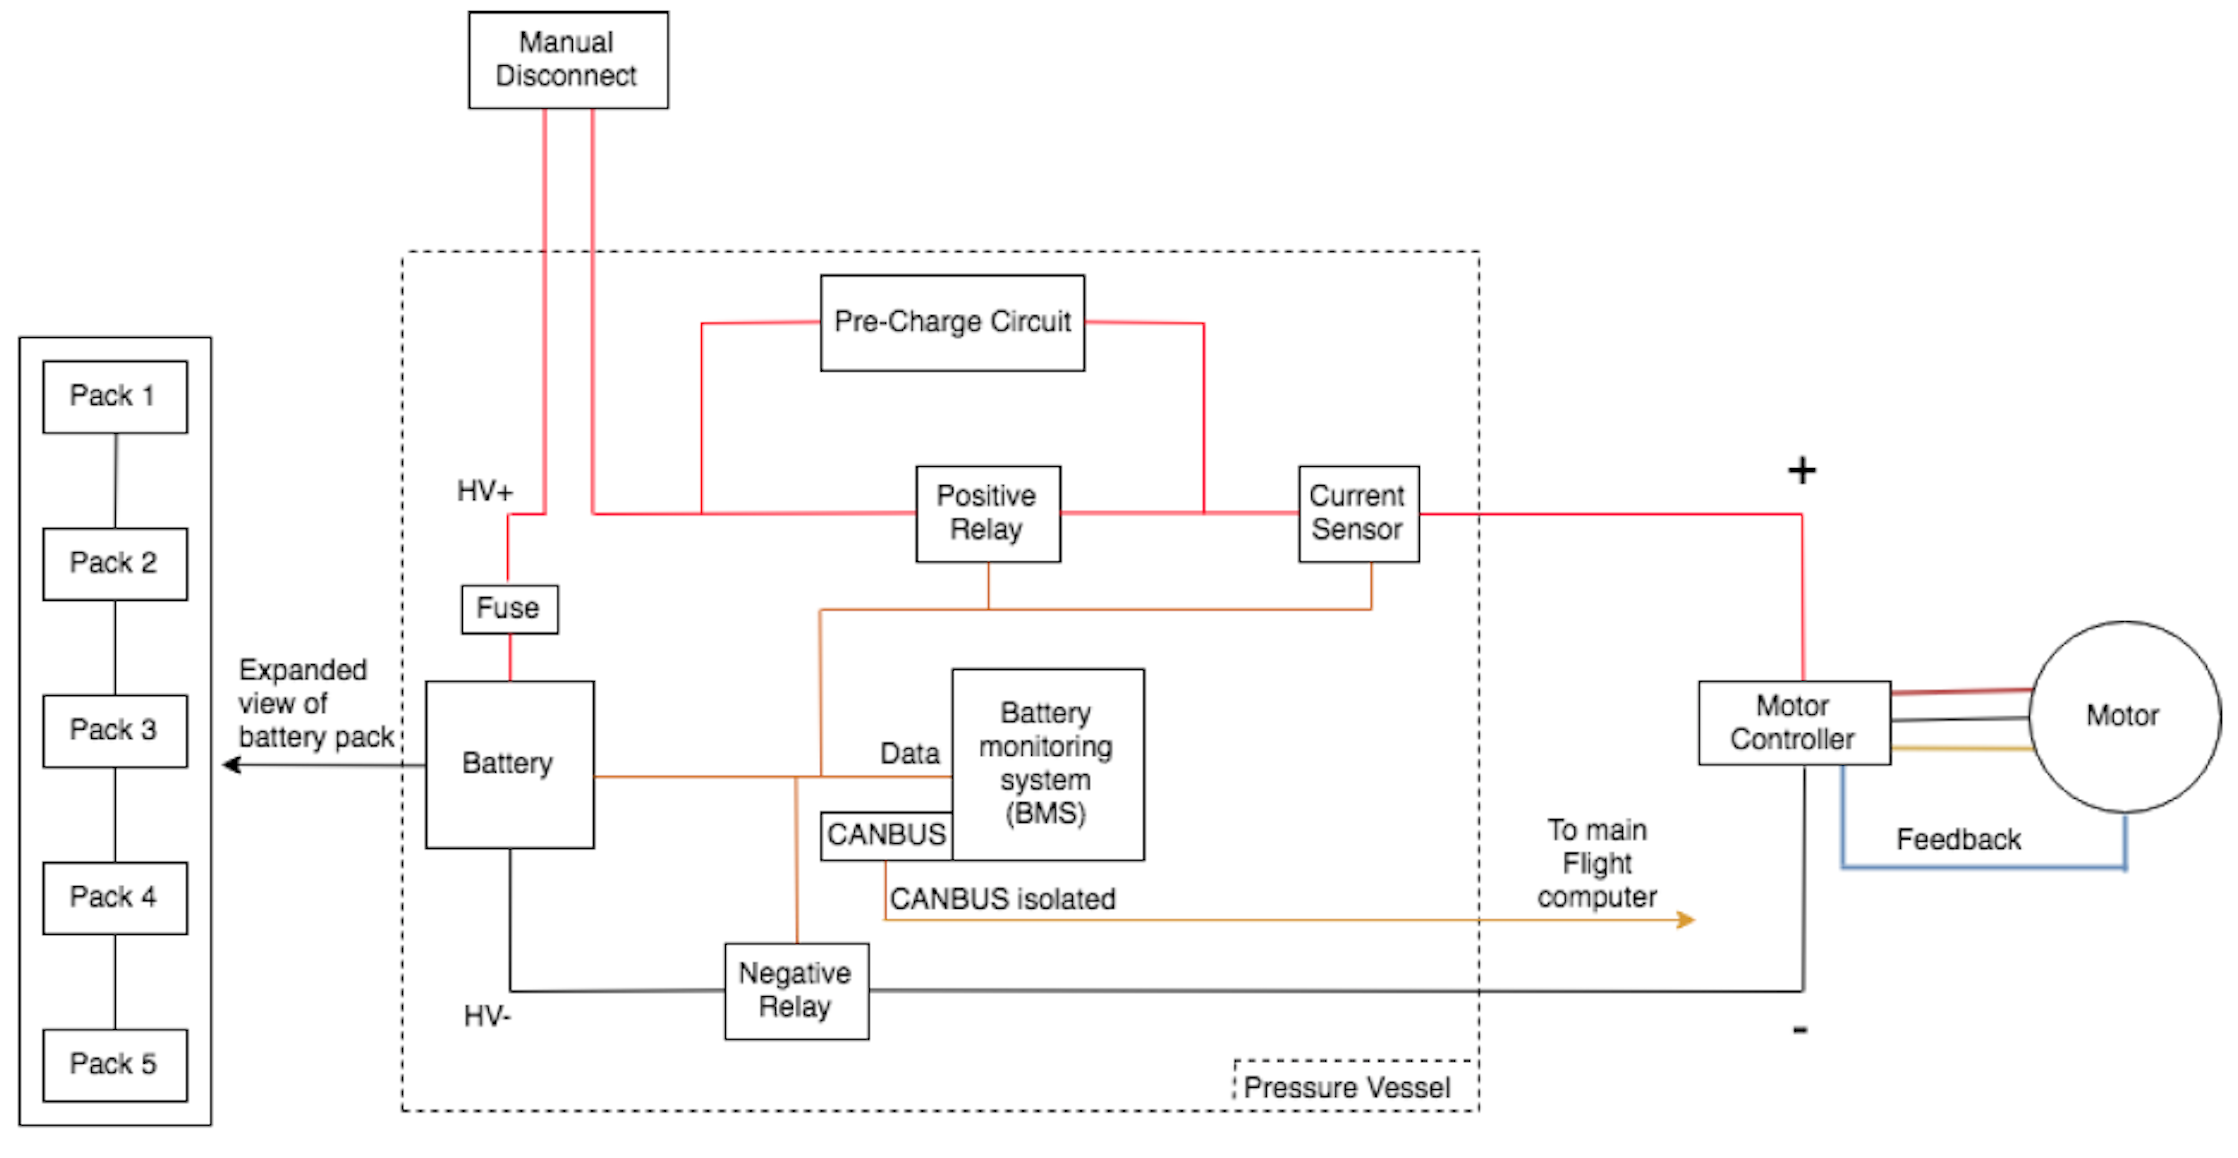
\includegraphics[width=1.0\textwidth]{fig/overview.png}
    \caption{Schematic of Propulsion System}
    \label{fig:schematic}
\end{figure}

The senior design team considered an idealised model of the propulsion system to estimate the power requirements and heat losses in a simulated run. A key assumption is that battery performance does not vary with temperature and current. The model assumes that the batteries always function at peak performance, and that the internal resistance of the batteries does not vary with temperature. Efficiency of the motor is determined by the torque and RPM. 

\pagebreak 

Figure \ref{fig:prop} contains plots of power supplied by the batteries and consumed by each component of the propulsion system during the run. The batteries have to supply up to $85\unit{kW}$ of power to the propulsion system to run the motor at peak performance. The difference between power supplied by batteries and consumed by the controller is dissipated in the form of heat. Integrating power loss over time, the total heat dissipated by the battery pack in one competition run is $300\unit{kJ}$.

\begin{figure}[!htb]
    \centering
    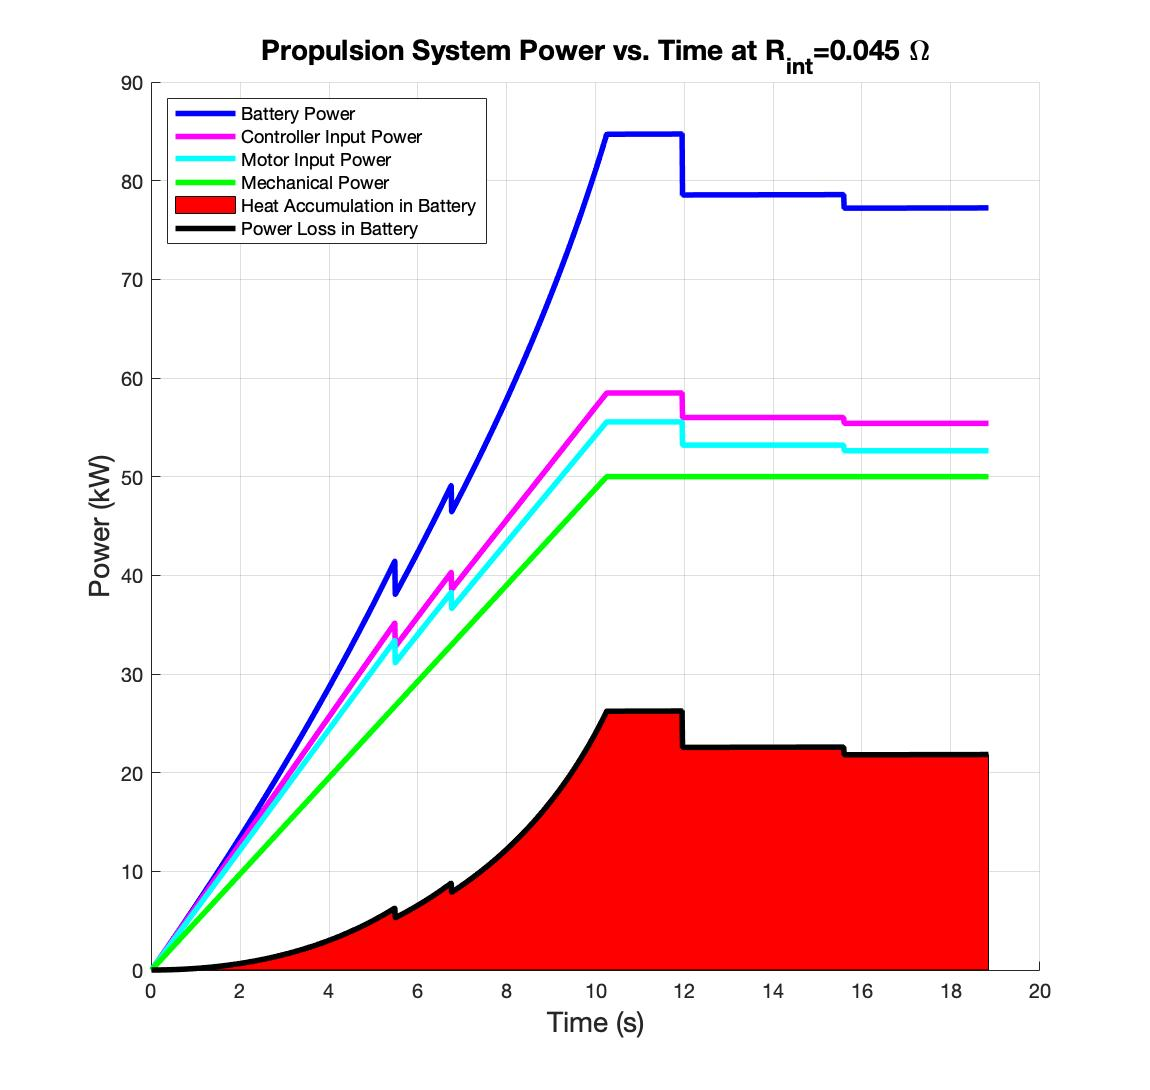
\includegraphics[width=0.8\textwidth]{fig/prop.jpg}
    \caption{Power Requirements of Components in the Propulsion System}
    \label{fig:prop}
\end{figure}

Figure \ref{fig:current} contains the plot of current supplied by the batteries over the course of the competition run. The current draw from the battery increases from $0\unit{A}$ to $800\unit{A}$ over approximately ten seconds. The current then holds constant for another ten seconds until the run is complete. Such short bursts of high amperage will strain the batteries and cause degradation. The jumps in power versus time and current versus time, plotted in Figures \ref{fig:prop} and \ref{fig:current}, respectively, occur due to sharp changes in the predicted efficiency curves of the motor.

\begin{figure}[!htb]
    \centering
    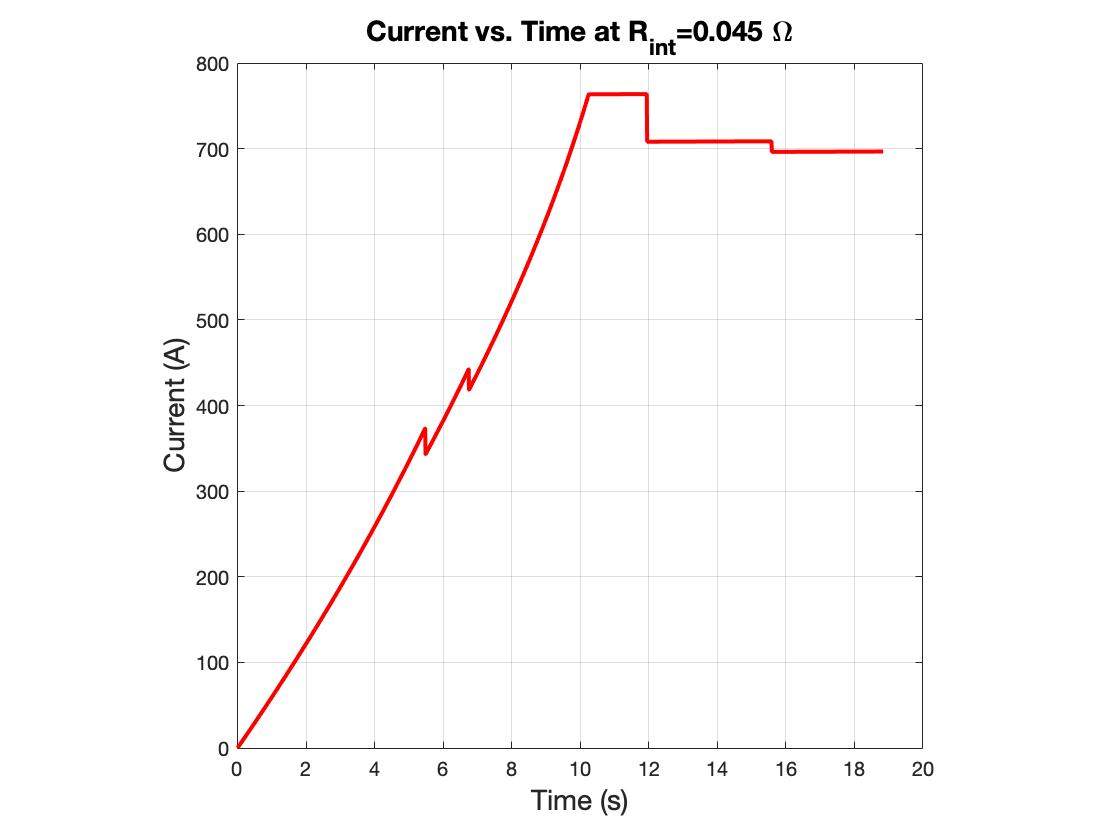
\includegraphics[width=0.9\textwidth]{fig/current.jpg}
    \caption{Current Supplied by Battery vs. Time}
    \label{fig:current}
\end{figure}

%========================================================================
\section{Design Considerations}
\subsection{Product Design Specification}

The design must consider all engineering specifications. The Project Design Specification (PDS) aims to narrow the scope of the project. Battery cooling designs for the Illini Hyperloop team and Novark Technologies can be judged with the following constraints.

\begin{enumerate}
    \item Performance
    
        The battery temperature must be kept under $50\unit{\degree C}$ for the duration of a single competition run, $20\unit{s}$. The run may be repeated up to three times with at least an hour intermission for pressurisation and depressurisation of the hyperloop tube. Cooling system must cool batteries $10-15\degrees\text{C}}$ while the tube is being depressurised. 
        
        
    \item Environment
     
        Ambient temperatures in Hawthorne, California range from $25-30\unit{\degree C}$ in August, when the competition is to be held. The absolute pressure of the battery box and its contents remain at 1 atmosphere (101 kPa). Ideally, the liquids must be noncorrosive and scale-free as to not impede heat transfer.
        
        
    \item Maintenance
        
        Cooling solution must be able to be cleaned or flushed to maintain heat transfer performance.
        
        
    \item Target Costs
      
        The research and development cost for the cooling solution must be under $\$1000$. Manufacturing cost is limited by the project sponsor, Novark Technologies. 
        
        
    \item Manufacturing Facility/Shipping
       
        Novark Technologies is to manufacture the cooling solution and ship it to Illini Hyperloop from Shenzhen, China. The lead time for shipping is 5--6 weeks.
        
    
    \item Packaging 
        
        The cooling solution is contained in a pressurised battery box.
    
    \pagebreak    
        
    \item Size
        
        The cooling solution must fit in the battery box which is a cylindrical pressure vessel with approximate dimensions 22\unit{in.} in length and 12\unit{in.} in diameter. The solution must also consider other components in the battery box, namely, the batteries, motor controller, battery controller, relays, and wiring. 
        
        
    \item Weight
        
        The total pod weight needs to be minimised for maximum speed. Therefore, the weight of the cooling solution must also be minimised.
        
        
    \item Aesthetics
        
        The cooling solution is covered by pressurised battery box. The interior layout of the battery box must be presentable in terms of neatness and functionality to SpaceX judges.
        
        
    \item Materials

        The primary material used in battery cooling solutions are aluminium and copper due to their high thermal conductivity. Most solutions also contain a coolant liquid with high heat capacity to act as a store for thermal energy. Common liquids used as coolants are water, and water-glycol mix. Rubber hosing may be used to connect the plate reservoirs. 
        
        
    \item Product Life Span
        
        The product is likely to remain in use for the duration of the Hyperloop competition, that is three runs.
        
        
    \item Standards, Specifications, and Legal Aspects
        
        Standards for the cooling solution include IEC 479-1, SAE J1811, and UL 1642.
        
        
    \item Ergonomics
        
        The filling procedure for coolant liquid into the cooling solution must be straightforward. The fill and drain locations of the cooling solution must be conveniently located for ease of run preparation. The cooling solution must also be easy to move in and out of battery box for access to internal components.
        
        
    \item Customer
        
        Illini Hyperloop wants a lightweight cooling solution to fit into existing design.
        
        
    \item Reliability and Quality
        
       Quality standards of $3\sigma$ must be followed with total production being one unit.
        
        
    \item Processes
        
        Novark Technologies uses patented design processes to manufacture cooling solutions.
        
        
    \item Timescales
        
        The lead times from Novark Technologies is 5--6 weeks including shipping time.
        
        
    \item Testing
        
        Testing for thermal profiles and internal resistance of the battery must be conducted to accurately model the heat generation of the batteries.
        
        
    \item Safety
        
        The batteries must be limited to $50\unit{\degree C}$ to stay within SpaceX regulations and prevent possible thermal runaway. The gauge of the wires must be adequate to handle maximum current.
        
        
    \item Company Constraints
        
        The team has access to Illini Hyperloop lab in the Nuclear Engineering Laboratory and fluid lab in Talbot Laboratory for testing and assembly purposes. 
        
        
    \item Patents, Literature, and Product Data
        
        Patents belonging to Novark Technologies are the only usable ones. The literature review details specifics about batteries and heat generations.
        
        
    \item Political and Social Implications
        
        Trading with China might be hampered by politics. Shipping time could increase if political complications arise. Socially, hyperloop pods have potential to change the entire transportation industry. 
        
        
    \item Disposal
        
        Aluminium or copper used in the cooling solution may be recycled. Water must not be contaminated with chemicals so that it can be reused or emptied into a public drain. The batteries may be recycled at the end of their life.
           
           
\end{enumerate}

\subsection{Broader Considerations}
Broader constraints involving public health, safety and welfare, as well as global, cultural, societal, environmental, and economic factors have been considered. The Hyperloop concept aims to revolutionise the world of transportation and broader impact of the senior design team's cooling solution must be considered. Advent of hyperloop-based public transportation systems may improve accessibility to public health services. Such transportation systems, much less prone to human error, should improve safety over automobile based transportation. Battery driven hyperloop systems, such as the one designed by Midwest Hyperloop, are prone to malfunctions and explosions. Battery explosions may cause bodily harm such as burns, and are reasons for safety and welfare concerns until a time when battery technology is perfected. The high velocity of $100\unit{m/s}$ that the Midwest Hyperloop pod is capable of travelling at may reduce commute time and increase productivity. The global, cultural, and societal factors of this project are all very similar.

With an effective cooling solution, hyperloop pods can connect cities, countries, and even continents. The possibilities will enhance global transport of both goods and passengers. Societies and cultures will have streamlined access to each other. The environmental factors of this project include looking at materials used for construction. Water is a renewable resource but the plates are made of metal. This metal can be recycled, but mining new materials has an environmental impact. Hyperloop as a method of travel is likely to be a much greener technology than current alternatives like air travel, changing the emissions of the rapid transit sector of transportation. Economic factors influenced by cooling relate to battery efficiency. The more efficient the cooling solution the more powerful the propulsion on the hyperloop pods can be, lowering the cost and increasing the speed. This economic pressure will likely have a ripple effect across the entire transportation industry.

%========================================================================
\section{Concept Selection}

The first step in designing a cooling solution was determining the cooling method that would be implemented. The team conducted brainstorming sessions and chose the three most viable options for further exploration. Those concepts are presented here. 

\subsection{Concept 1: Phase Change Material}
In the case of phase change materials (PCM), the phase change temperature of the material matches the temperature at which cooling is required. As the material changes phase it removes heat from the source while keeping the temperature constant. The temperature climbs to a certain value and is held constant as the material absorbs latent heat for complete phase change before the temperature climbing again.


Illini Hyperloop initially proposed to use PCM as a cooling solution, but the SP50 Rubitherm material, as shown in Figure \ref{fig:RubithermSP-50}, has a phase change temperature of 50\degrees C. The SP50 results in the batteries operating at the highest point of their operating range for a majority of their run, hurting their service life. Operating at such temperatures also poses a safety risk to the pod as the high temperatures may result in the batteries catching fire or exploding.

\begin{figure}[!htb]
 \centering
	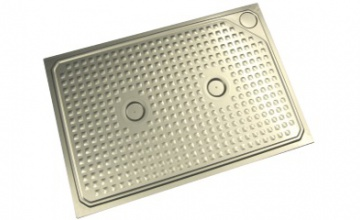
\includegraphics[width=0.9\textwidth]{final/fig/CSM_400x240.jpg}
    \caption{Rubitherm SP-50}
    \label{fig:RubithermSP-50}
\end{figure}

 The biggest issue with the PCM cooling solution is performance. The PCM systems have limited super cooling restricted to 2\degrees C to 3\degrees C. Limited super cooling lowers the possible temperature gradient that can be introduced in the system which further dictates the rate of flow of heat. 

\subsection{Concept 2: Passive Liquid Cooling}
Passive liquid cooling uses a working liquid cooled to low temperatures and contained within a conductor to draw heat away from the source. Channels are machined into thermally conductive metals, as shown in Figure \ref{fig:Passive Cooling Plate}, and then these plates are used to sandwich the battery pack. The system is passive because there is no forced fluid flow during cooling.

The implementation of passive liquid cooling system requires each battery pack to be placed between two vacuum brazed cold plates. These cold plates are flushed with a refrigerant prior to the pod's run. This induces a very high thermal gradient between the cold plates and the working fluid, allowing for rapid removal of heat from the batteries---thereby keeping them well below the upper reaches of their operating temperature.

\begin{figure}[!htb]
 \centering
	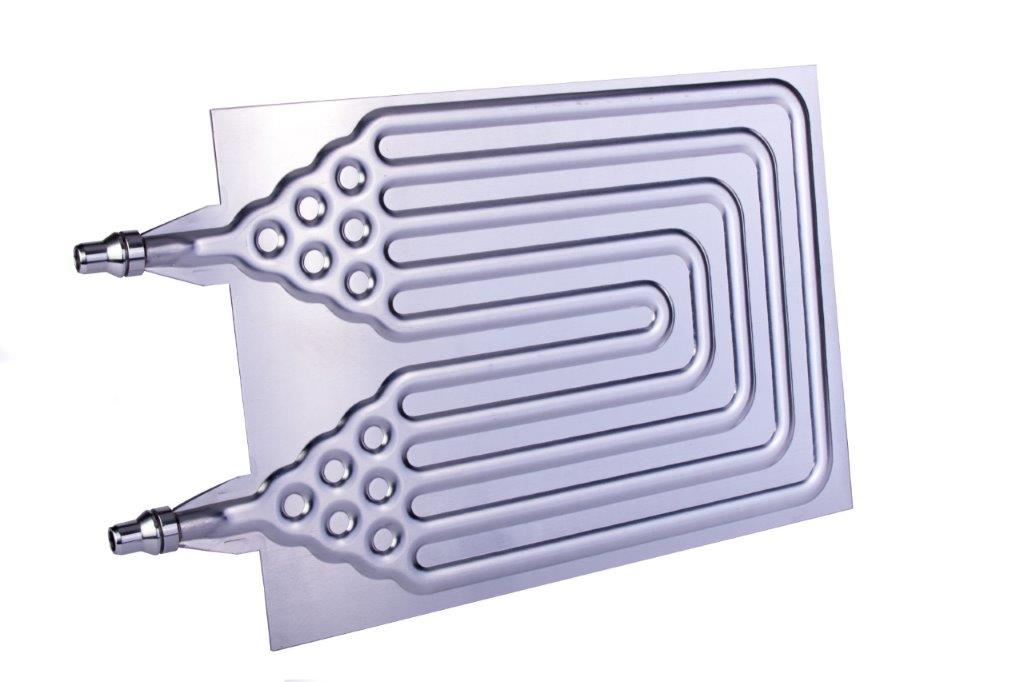
\includegraphics[width=0.8\textwidth]{final/fig/Plate.jpg}
    \caption{Passive Cooling Plate}
    \label{fig:Passive Cooling Plate}
\end{figure}

The short run times of the hyperloop pod eliminates the need for flow of the working fluid. Having the liquid sit in the channels is sufficient to remove heat from the batteries. Without a pump or a reservoir that would otherwise be required in an active liquid cooling system, a passive system is much lighter and more compact.
%\begin{figure}
%\centering
%	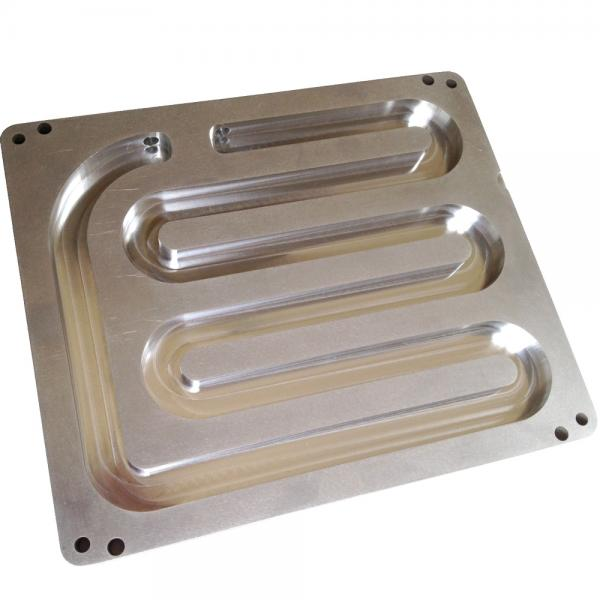
\includegraphics[width=0.5\textwidth]{proposal_template_v0.2/fig/chill.jpg}
%\caption{Passive Cooling Plate}
%\label{fig:Passive Cooling Plate}
%\end{figure}

\subsection{Concept 3: Active Liquid Cooling}
Active liquid cooling uses principles similar to passive water cooling in addition to circulating the working fluid in a closed loop. Fluid circulation requires a pump and a reservoir as shown in Figure \ref{fig:Active Liquid Cooling}. By pumping the fluid throughout the loop, the temperature of the fluid can be assured to be close to its initial temperature---keeping the thermal gradient and the heat flow out of the batteries constant across the whole run.

In terms of heat transfer performance, the active liquid cooling system is better than the passive liquid system. This is due to the fact that the convective heat transfer coefficient increases with higher fluid velocities. The improved performance comes at the cost of including a reservoir and a pump, which add bulk and weight to the cooling solution. The pump also requires power, which will further load the battery pack. 

\begin{figure}[!htb]
 \centering
	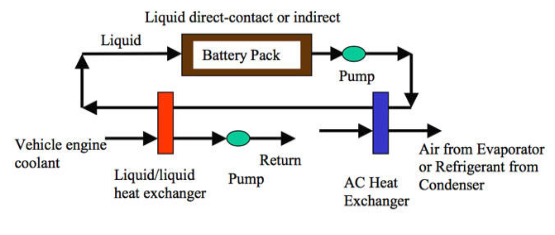
\includegraphics[width=0.8\textwidth]{final/fig/active_cooling.png}
    \caption{Active Liquid Cooling}
    \label{fig:Active Liquid Cooling}
\end{figure}

\subsection{Concept Selection}
A decision matrix was used in order to validate the best concept to moving forward. Concept 2---passive water cooling---shows the highest score and therefore the highest potential for design success. The temperature of the system is too variable to get consistent cooling from the PCM. The idea of PCM is thus discarded as the poor cooling rate per unit volume does not outweigh the advantages. The drawbacks of weight and power consumption, along with the short run time of the system, resulted in the active liquid cooling concept being dropped in favour of the passive liquid system.

\begin {table}[h]
  \centering  \caption{Decision Matrix}
  \label{figure:matrix}
	\begin{tabular}{r | r | c || c c c}
		\multicolumn{2}{r}{Criteria}	&Weight Factor	&Concept1	&Concept2	&Concept3 \\
		\hline
		\multirow{3}{*}{Mechanical}	
			&Temperature Control	&5	&3	&4	&5	 \\
			&Weight		&4	&5	&4	&3	 \\
			&Size			&4	&2	&3	&2	 \\ 
			\hline
		\multirow{4}{*}{Other}	
			&Customer Preference		&4	&2	&4	&2	 \\
			&Manufacturing Cost	&3	&4	&3	&2	 \\
			&Maintenance	&2	&3	&3	&1	 \\
			&Aesthetics		&1	&2	&3	&2	 \\ 
        \hline
		\multicolumn{3}{r}{\textbf{Total Score}}	&71		&82					&63		
	\end{tabular}	
\end{table}



%========================================================================
\section{Battery Testing}\label{battery_testing}

The senior design team purchased a single $22.2\unit{V}$ Li-Po battery for the purposes of testing. As Li-Po batteries are inhomogeneous bodies, its components do not heat up evenly. The team located regions of localised heat concentration, or hot spots, as these regions are susceptible to overheating. The thermal profile test was performed twice for redundancy. On the third test, the battery failed. 

\subsection{Thermal Profile Test}\label{profile-test}
The battery was placed in an infrared isolating shield and loaded by a high power resistor. The surface temperature of the battery was monitored by a thermal camera as it passed currents of currents up to $100\unit{A}.$ The experiment is setup as shown in Figure \ref{fig:Battery Test Setup}. The battery dissipated $6\unit{kJ}$ of heat over the $60\unit{s}$ test.

\begin{figure}[!htb]
 \centering
	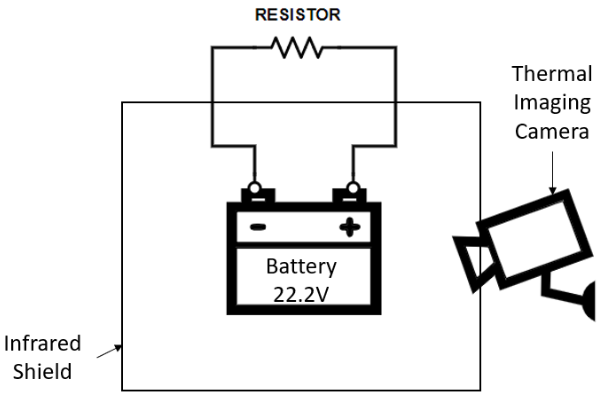
\includegraphics[width=0.5\textwidth]{final/fig/Test_Setup.png}
    \caption{Battery Test Setup}
    \label{fig:Battery Test Setup}
\end{figure}

The battery was photographed at ambient temperature as shown in Figure \ref{fig:Battery Thermal Profile 0} and $60$ seconds after loading, as shown in Figure \ref{fig:Battery Thermal Profile 6}. Hot spots formed bands in the lateral direction of the battery as shown in Figure \ref{fig:Battery Thermal Profile 6}.

The thermal profile test serves as a qualitative measure to identify trends in heat concentration on the battery surface. However, as Li-Po batteries are covered in a plastic insulating jacket---shown in Figure \ref{fig:batteryjacket}---and most of the heat produced is trapped in the inside of the battery. Temperature measurements may only be made on the surface of the battery as performing invasive tests on Li-Po batteries may pose safety risks. Further, the trends in heat generation may not necessarily be the same at target currents of $800\unit{A}$. The results of this test will aid in the design of cooling geometry based on the areas of major heat concentration and hence requiring the most cooling.
 
\begin{figure}[!htb]
     \centering
     \begin{subfigure}[b]{0.49\textwidth}
         \centering
         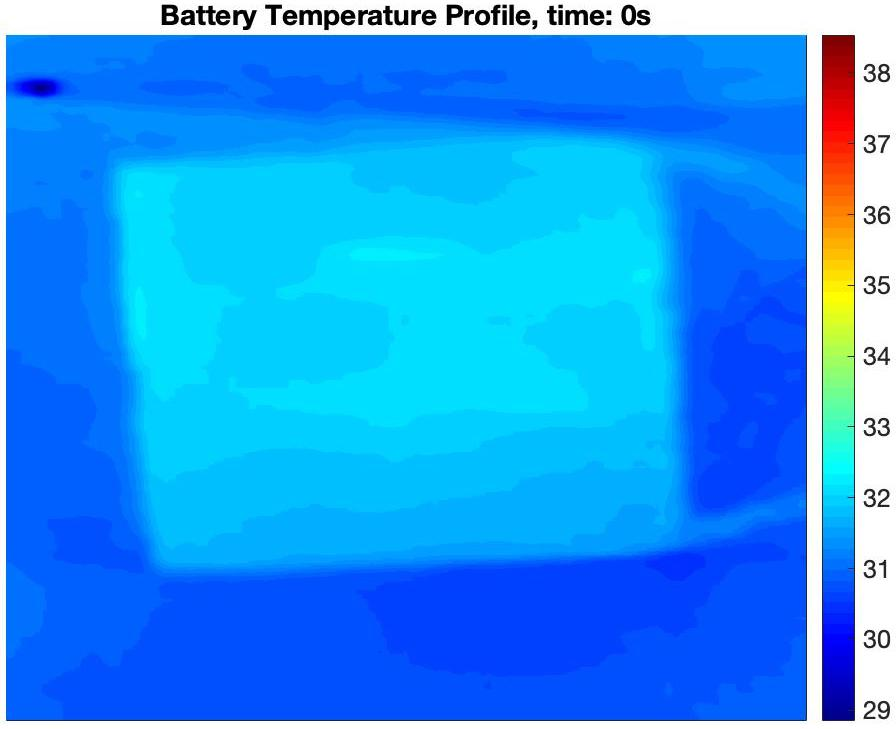
\includegraphics[width=\textwidth]{final/fig/profile0.jpg}
         \caption{Battery Thermal Profile at $T=60\unit{s}$}
         \label{fig:Battery Thermal Profile 0}
     \end{subfigure}
     \hfill
     \begin{subfigure}[b]{0.49\textwidth}
         \centering
	     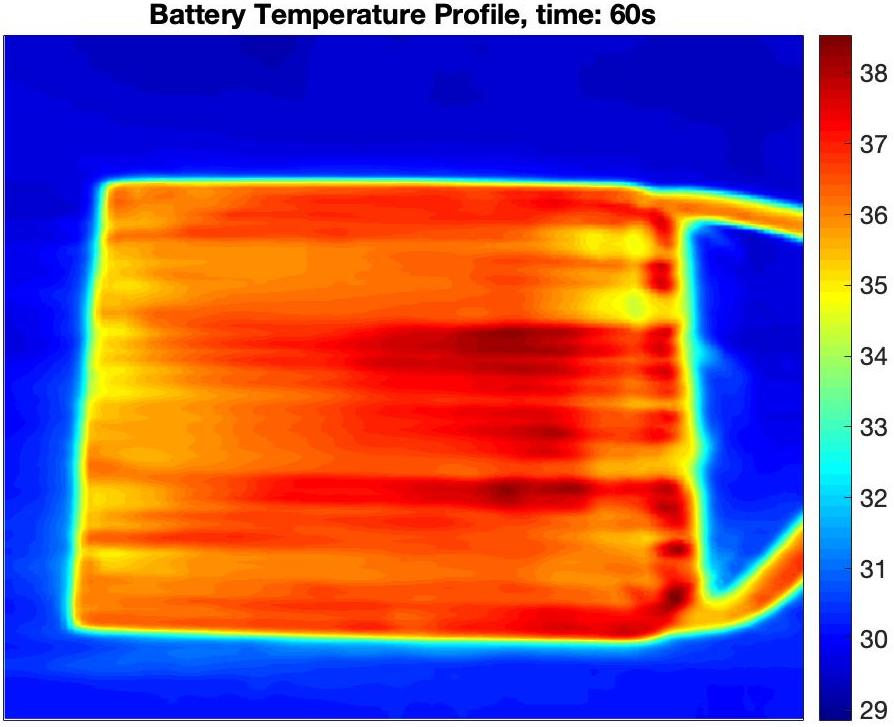
\includegraphics[width=\textwidth]{final/fig/profile6.jpg}
         \caption{Battery Thermal Profile at $T=60\unit{s}$}
         \label{fig:Battery Thermal Profile 6}
     \end{subfigure}
     \caption{Battery Thermal Profiles}
\end{figure}

\begin{figure}[h!]
 \centering
	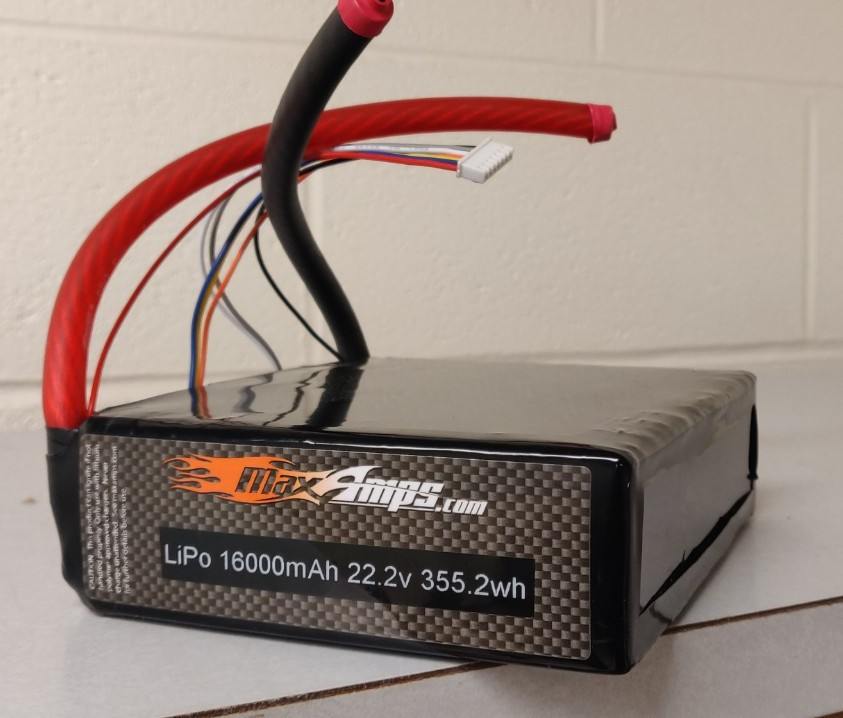
\includegraphics[width=0.7\textwidth]{final/fig/batteryjacket.jpg}
    \caption{Battery Insulating Jacket}
    \label{fig:batteryjacket}
\end{figure}

\pagebreak

\subsection{Failure During Testing}
In reproducing the test in Section \ref{profile-test} surface temperature profile testing the battery was loaded repeatedly for three runs without recharging the battery. Consequently, the battery was unbalanced and some of the $24$ cells were strained, damaging the battery irreversibly. In Figure \ref{fig:Battery Thermal Profile Failure}, the cells on one side of the battery can be seen to be over-heated.

\begin{figure}[h!]
 \centering
	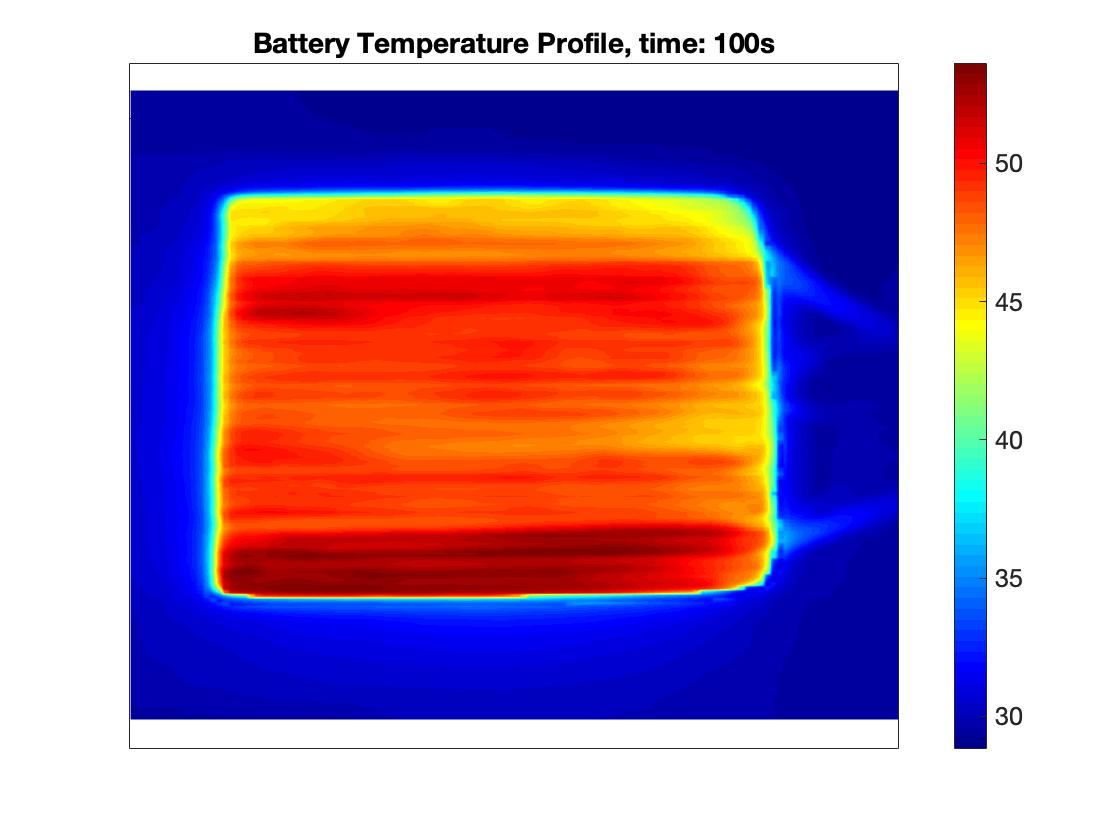
\includegraphics[width=0.7\textwidth]{final/fig/profilefail.jpg}
    \caption{Battery Thermal Profile at Failure}
    \label{fig:Battery Thermal Profile Failure}
\end{figure}


%========================================================================
\section{Battery Box}
Li-Po batteries are covered in a soft plastic shell, and may not be operated in the vacuum conditions of a hyperloop tube. The current design proposes that the battery pack be stored in a pressurised battery box maintained at $1\unit{atm}$ pressure. The battery box is made of aluminium to keep it lightweight. The battery box, shown in Figure \ref{fig:Battery Box}, is a cylindrical in shape to avoid stress concentrations at the corners. The limited space available in the hyperloop chassis constrained the size of the battery box. The inside of the pressure vessel can be accessed from one of the flanged caps. The battery box is fitted with a pressure-release valve to prevent buildup of excess pressure in the system.

\begin{figure}[!htb]
     \centering
     \begin{subfigure}[b]{0.49\textwidth}
         \centering
	    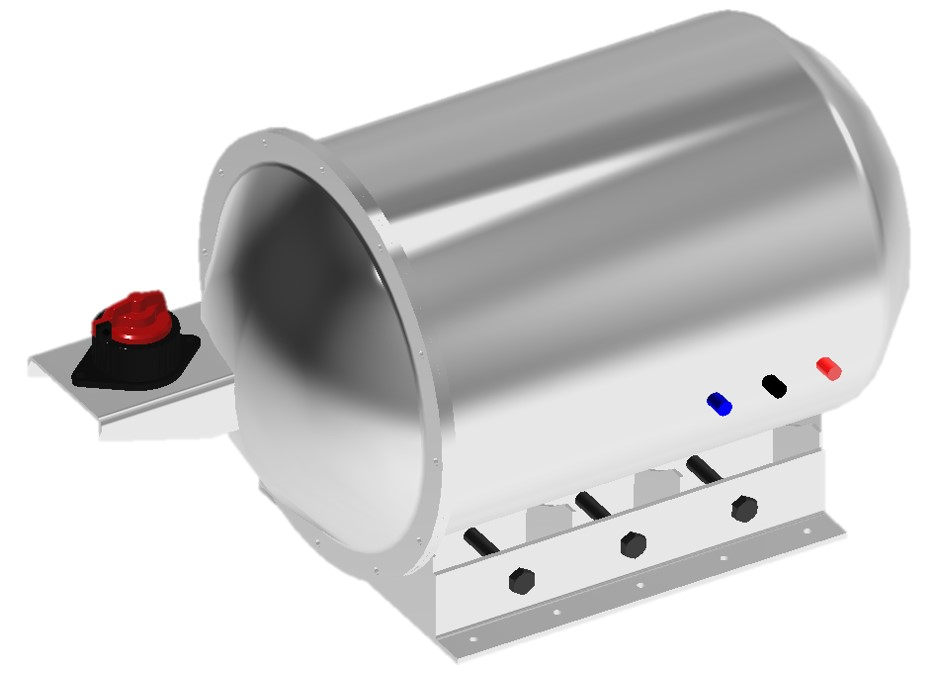
\includegraphics[width=\textwidth]{final/fig/batterybox1.jpg}
        \caption{Battery Box}
        \label{fig:Battery Box}
     \end{subfigure}
     \hfill
     \begin{subfigure}[b]{0.49\textwidth}
         \centering
	    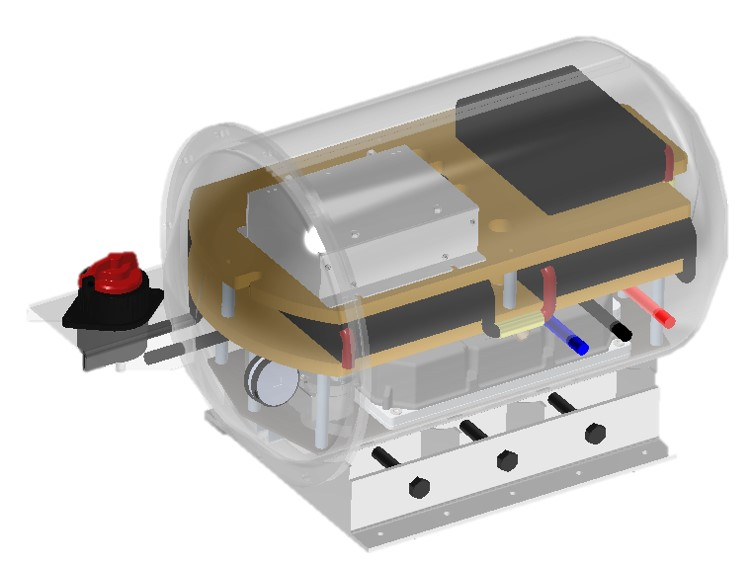
\includegraphics[width=\textwidth]{final/fig/batterybox2.jpg}
        \caption{Battery Box Internals}
        \label{fig:internals}
     \end{subfigure}
     \caption{Battery Box}
\end{figure}

The cooling solutions must fit within the space and weight constraints of the battery box. The motor controller, battery controller, and safety fuse are also stored within the battery box to reduce electrical losses. The cooling solution is made into the battery box so that batteries can be stacked without causing interference problems. Four of the five batteries are pressed between the two plates, while the fifth rests on top of the top plate. The configuration minimises the length of cables to $900\unit{mm}$ connecting all batteries in series. Shorter wires decrease resistance and power loss and improve efficiency. All electrical wiring used is AWG $4$ gauge. Four batteries have two surfaces in contact with cooling plates, and one has a single surface. The imbalance is due to a lack of space for an additional cooling plate for the isolated battery. The battery box was constrained in radius and length by the chassis of the pod. Recommendations to mitigate the effects of this imbalance are made in Subsection \ref{reco-plate}. The battery box can be seen in \ref{fig:Battery Box} along with the location of the cooling plates and batteries in Figures \ref{fig:internals} and \ref{fig:batteries and plates}.

\begin{figure}[h!]
 \centering
	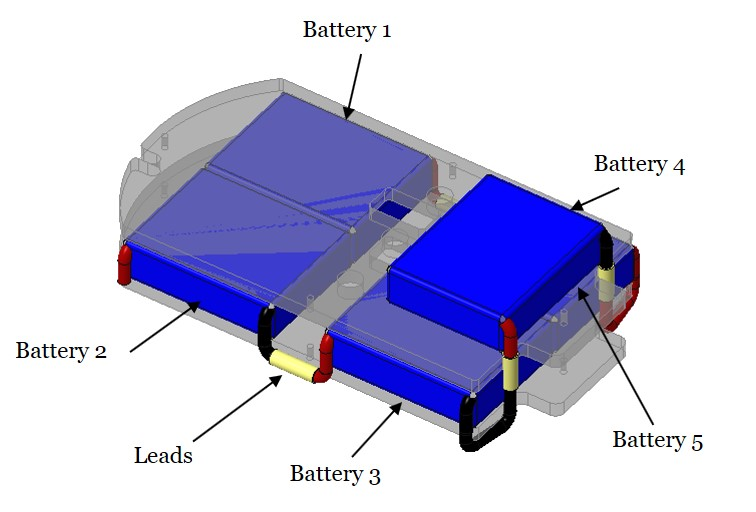
\includegraphics[width=1.0\textwidth]{final/fig/batterybox3.jpg}
    \caption{Battery Locations}
    \label{fig:batteries and plates}
\end{figure}

%========================================================================
\section{Cooling Plates}
In consultation with Novark Technologies, the senior design team designed a passive liquid cooling solution for the hyperloop batteries. Heat produced in the batteries would be dissipated into coolant-filled metal plates fabricated by Novark Technologies. To decrease thermal resistance between the cooling plates, and the batteries, and to increase the heat flux from the batteries into the plates, thermal paste may be applied at the battery plate interfaces to reduce contact resistance. The cooling plates were constrained by the size constraints imposed on the battery box. The cooling plates are designed to absorb $300\unit{kJ}$, the upper estimate of heat generated in the battery pack. As heat flow from the battery to the plates is proportional to the difference in temperature, it is imperative to maintain the region of plates in contact with the batteries relatively cool. A high conducting metal would be able to carry quickly carry heat from hot regions of the plates. A large surface area at the water-aluminium interface would further improve heat transfer from aluminium into water.

Fins have been added in the interior of the plates. Fins increase surface area at the coolant-metal interface, and create channels down which the coolant can flow. Further, fins help in carrying heat away the metal surface in contact with the battery to regions in the interior of the plate. However, fins take up volume which could otherwise be used for water, reducing the overall heat capacity of the plates. Thus fins are only implemented within the plates in the areas directly in contact with a battery, which need to be maintained at lower temperatures. As a consequence of the tests performed in subsection \ref{profile-test}, batteries are oriented such that the high temperature bands seen in Figure \ref{fig:Battery Thermal Profile Failure} are perpendicular to fin direction. The orientation of the fins along the length of the plate further facilitate fluid flow throughout the whole system for filling and emptying.

Water was chosen to be the liquid coolant as it has the highest specific heat of any common liquid. In addition, the temperature range of the system will not exceed either the freezing or boiling point of water. On the recommendation of Novark Technologies, the plates were manufactured with aluminium due to its high conductivity. The plate height, shown in Figure \ref{fig:findim2}, is obtained by calculations in Subsection \ref{coolant_vol} ensuring that the volume of water exceeds the minimum required, when starting from an initial temperature obtained in Subsection \ref{initial_tem}.

\begin{figure}[!htb]
 \centering
	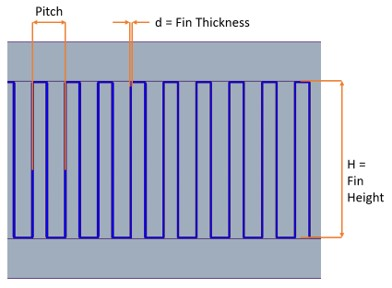
\includegraphics[width=.5\textwidth]{final/fig/fin_dimensions.jpg}
    \caption{Internal Fin Dimensions Cross Section}
    \label{fig:findim2}
\end{figure}

The minimum surface area of fins required was computed based on calculations in Subsection \ref{fin-area}. Fin parameters such as pitch, and thickness---shown in Figure \ref{fig:findim2}---were selected from \cite{novark}, and length, width---shown in Figure \ref{fig:findim1}---based on battery dimensions such that the surface area at the water-aluminium interface exceeds the minimum surface area required. Allowable fin pitch and thickness values shown in Figure \ref{fig:findim2}. were obtained from \cite{novark}. Length and width of finned regions is determined by the battery configuration.

\begin{figure}[!htb]
 \centering
	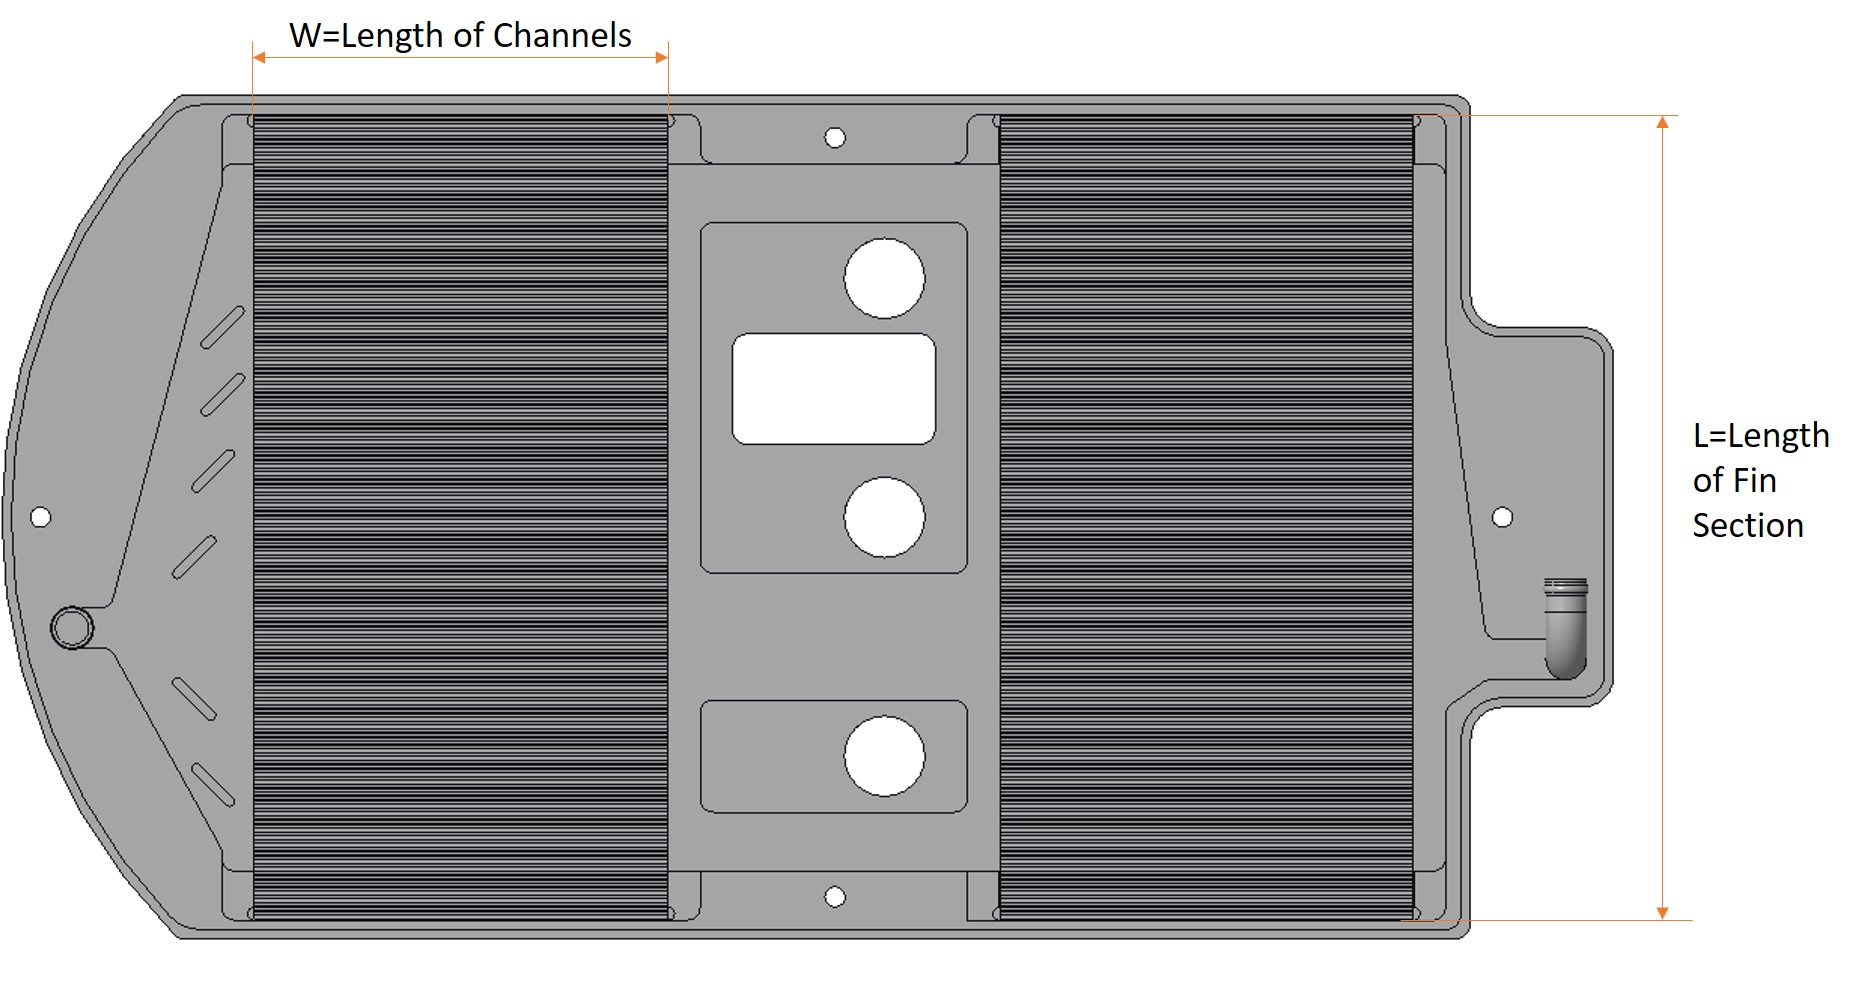
\includegraphics[width=0.7\textwidth]{final/fig/fin_dimensions2.jpg}
    \caption{Internal Fin Dimensions Top View}
    \label{fig:findim1}
\end{figure}

A few holes are machined through each plate in order to accommodate wire routing, plate support, and access to components below the plates. The four small holes around the edge of the plate allow for support attachments. The three larger holes in the centre facilitate access to lower connections to the motor controller connections. The large square hole is made for wiring connections between the motor controller and the battery controller. A fitting is added on each end of the plates to allow for filling and emptying. The tubing on the plates is $0.50\unit{in}$ in diameter which allows for $0.50\unit{in}$ rubber hoses to be used on the system. The fittings in the back, seen in Figure \ref{fig:fittings}, will connect the plates so that the two plates can act as one continuous pipe. An image of the delivered product is shown in Figure \ref{fig:plates}.


% The dimensions of the cooling plates are as follows: overall length is $507.16\unit{mm}$, overall width is $266.7\unit{mm}$, overall thickness is $18\unit{mm}$. The final specifications for all four sets of fins are as follows: length of fin section is $253.75\unit{mm}$, length of channels is $130\unit{mm}$, pitch of fins is $2.5\unit{mm}$, height of fins is $12\unit{mm}$, and fin thickness is $0.15\unit{mm}$. The total fin surface area is $0.68\unit{m^2}$ which is more than the minimum required by the high flux region which is $0.60\unit{m^2}$ and significantly greater than the required surface area in the low flux regions which is $0.30\unit{m^2}.$ The thickness and pitch are the minimum allowed by manufacturing constraints. This total area of fins allows heat to be transferred from the plates to the water more effectively. 

\begin{figure}[!htb]
    \centering
    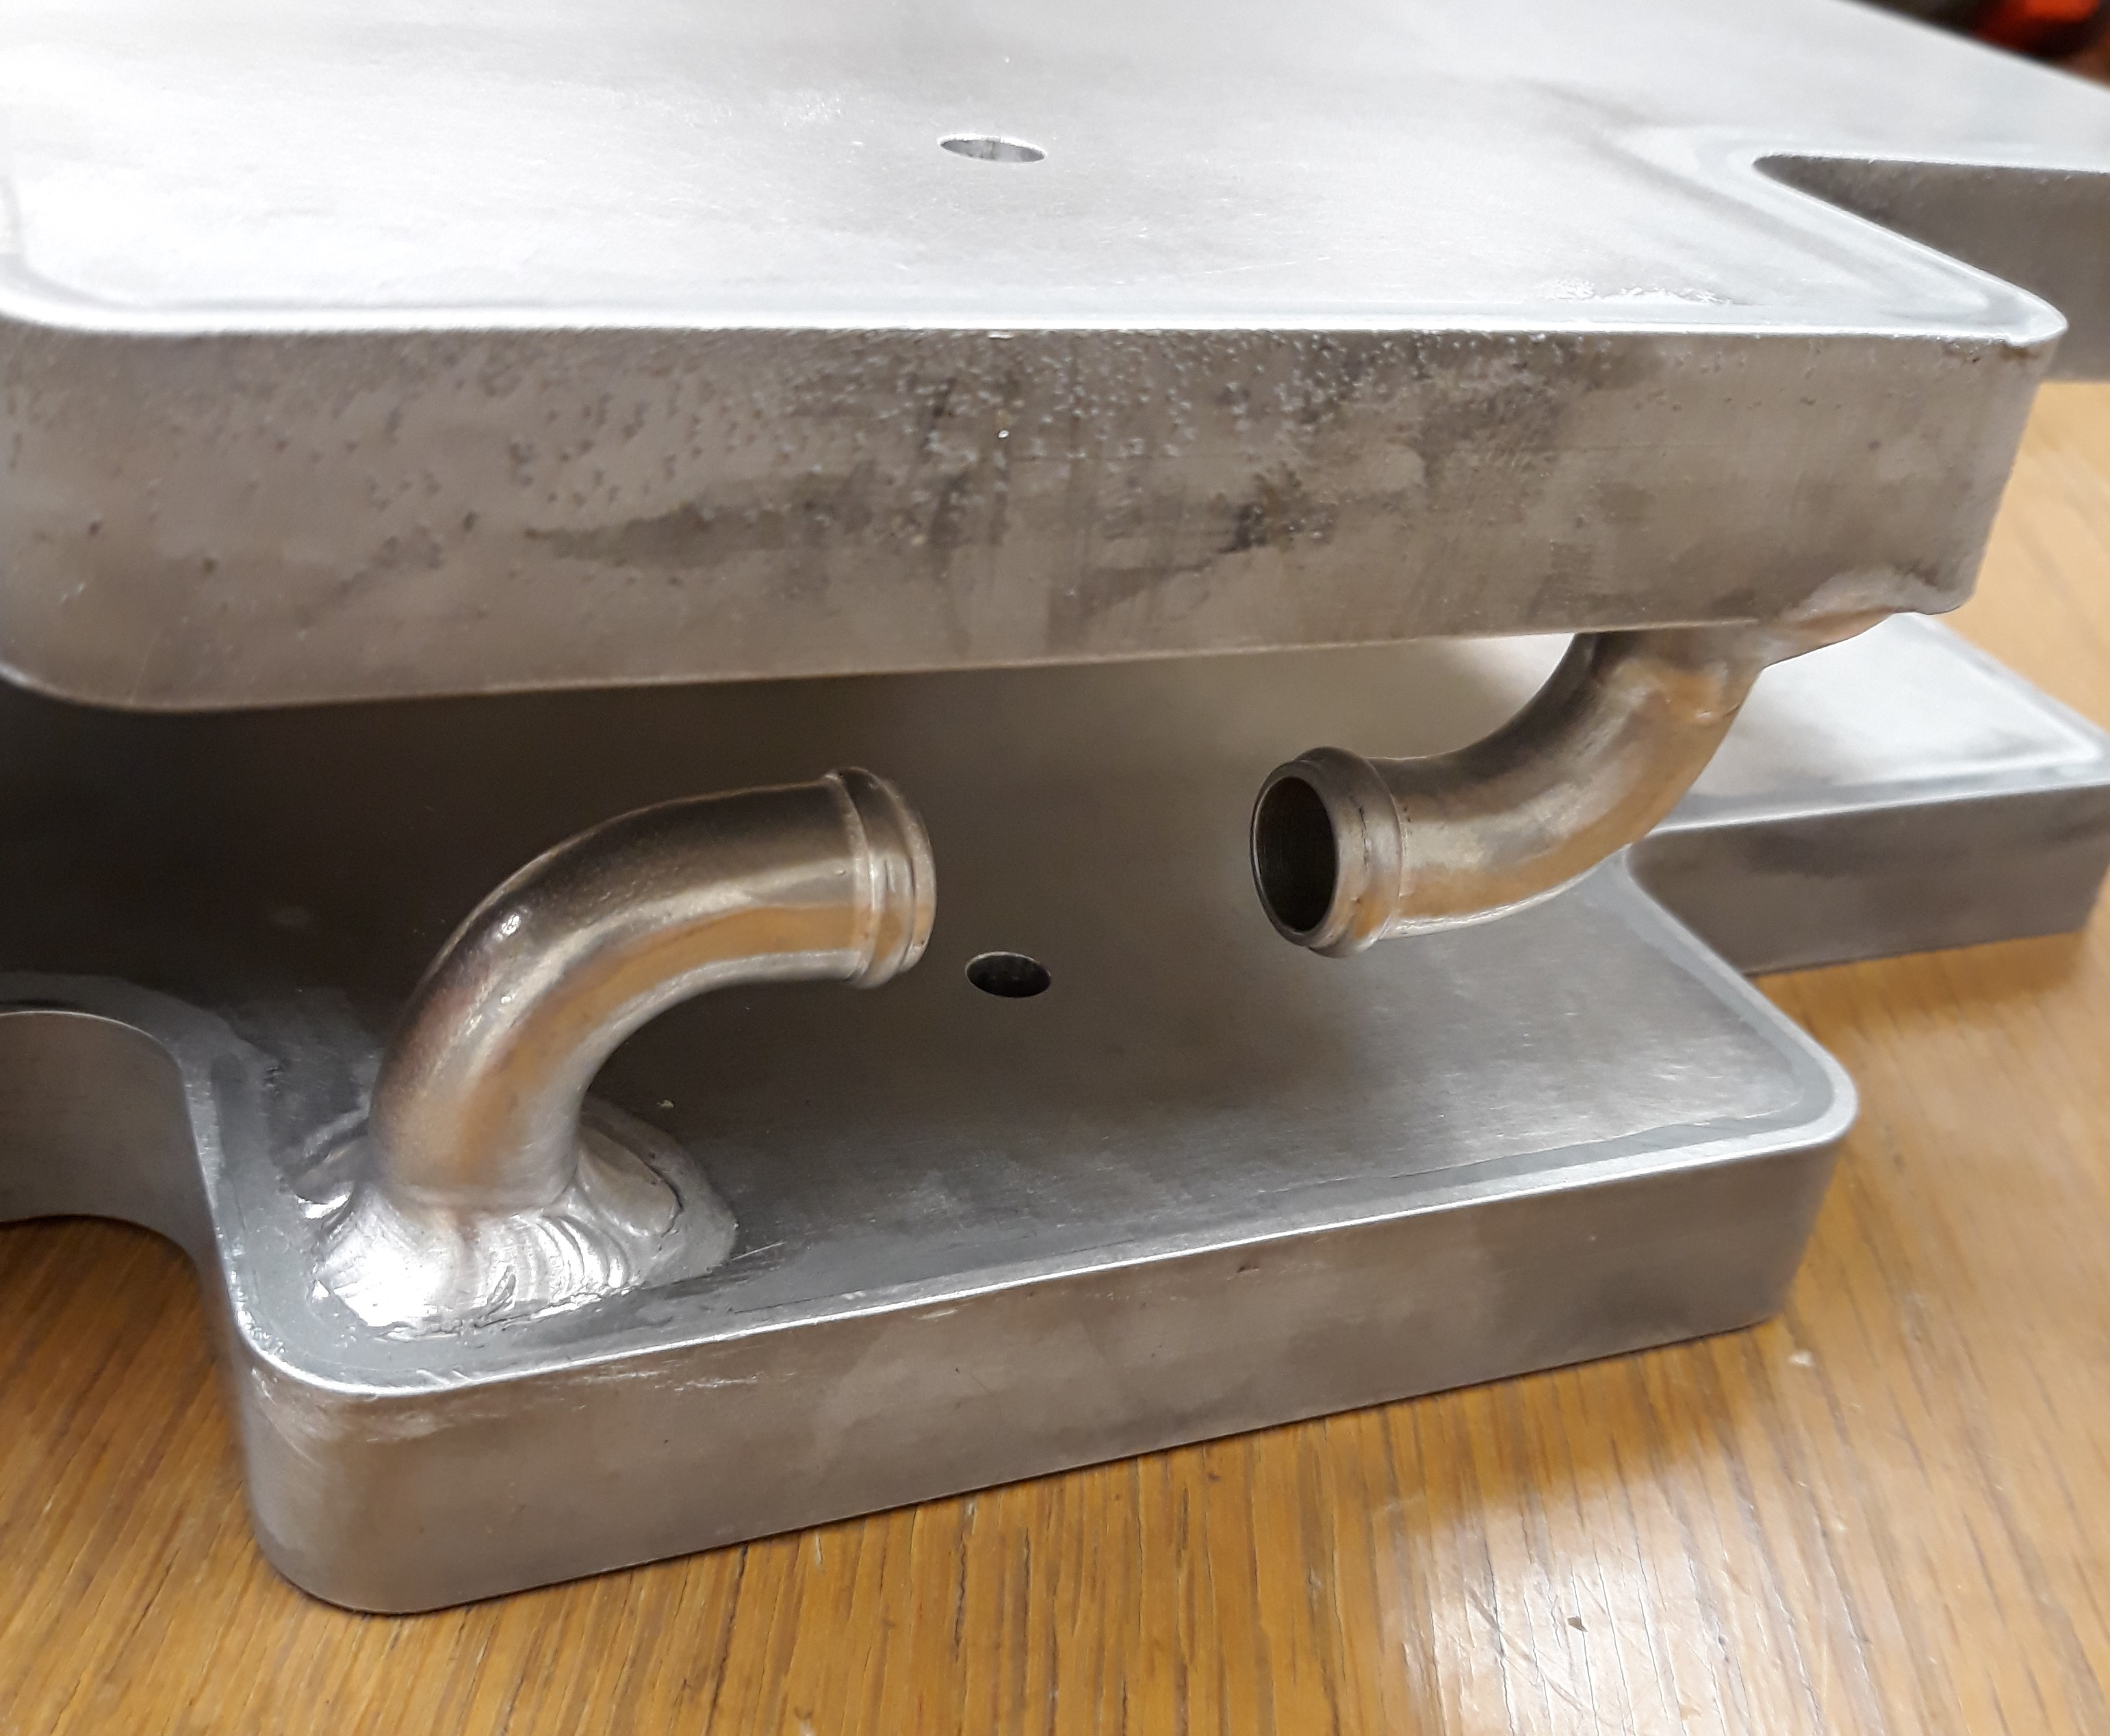
\includegraphics[width=0.5\textwidth]{final/fig/fittings.jpg}
    \caption{Pipe Fittings for Hose Attachment}
    \label{fig:fittings}
\end{figure}
 
\begin{figure}[!htb]
 \centering
	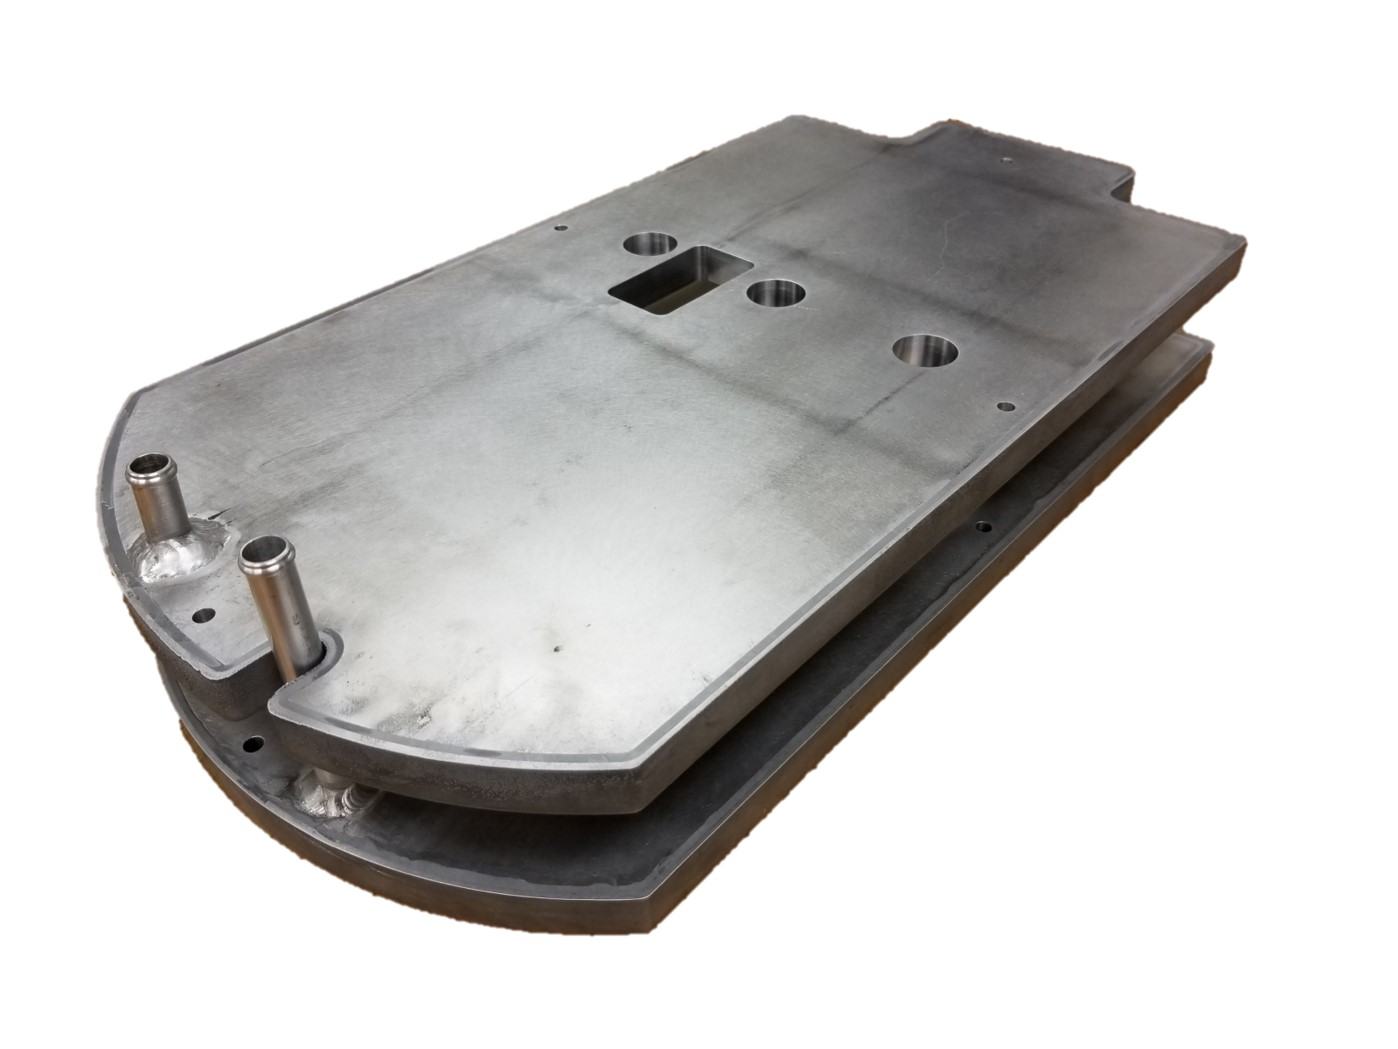
\includegraphics[width=0.9\textwidth]{final/fig/thermal_plates.jpg}
    \caption{Aluminium Brazed Plates}
    \label{fig:plates}
\end{figure}
%========================================================================
\section{Analysis}
The senior design team verified the ability of the cooling plates to absorb $300\unit{kJ}$ of heat by performing finite element analysis using Ansys\textsuperscript{\textregistered}. It is imperative that the plates diffuse heat away from the batteries so that the battery-plate interface remains cool to allow for heat transfer from battery to the plate. The boundary conditions used for the top plate were as follows: heat flux of $145\unit{kW/m^{2}}$ to the top surface corresponding to the are of contact with the single battery, heat flux of $72\unit{kW/m^2$} to the bottom surface corresponding to the area of contact with the four batteries and a convective heat transfer coefficient of $750\unit{W/m^2K}$. The mesh generated for the top plate consisted of $234,933$ linear tetrahedral elements. The boundary conditions for the middle plate were as follows: heat flux of $72\unit{kW/m^2}$ to the top surface, corresponding to the area of contact with the 4 batteries and a convective heat transfer coefficient of $500\unit{W/m^2K}$. The mesh generated for the top plate consisted of $236,423$ linear tetrahedral elements.

\begin{figure}[!htb]
    \centering
    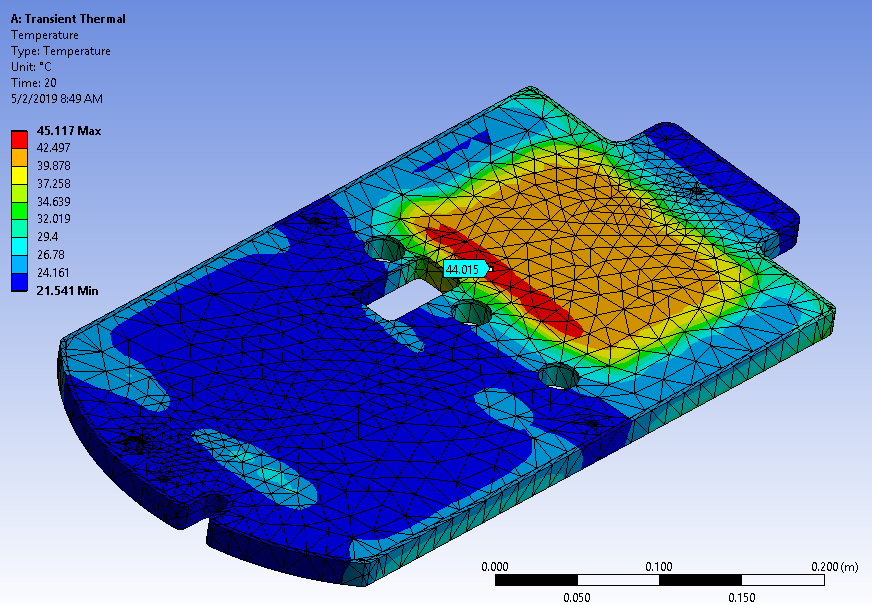
\includegraphics[width=0.8\textwidth]{final/fig/Top_Plate_1.png}
    \caption{Thermal Profile of Top Plate Cover}
    \label{fig:Top_Plate_1}
\end{figure}

\begin{figure}[!htb]
    \centering
    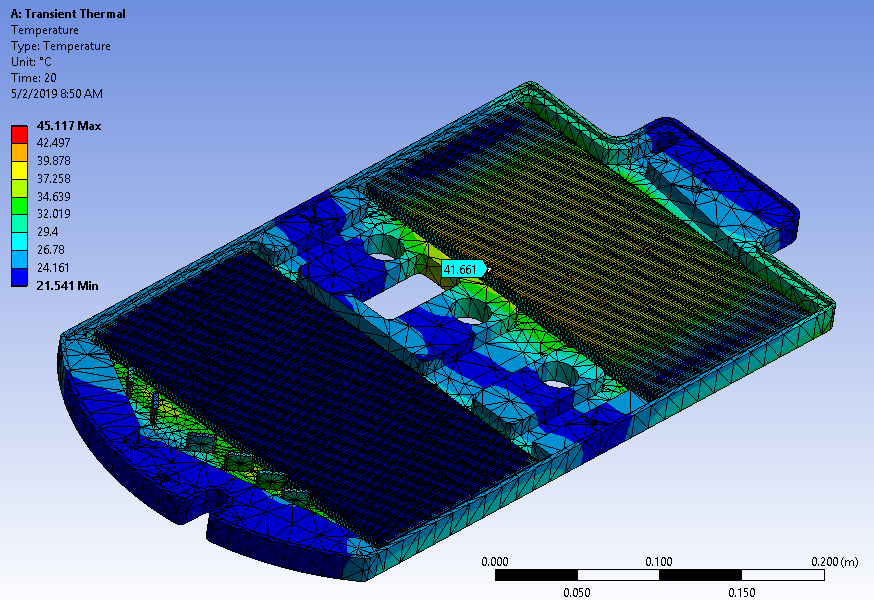
\includegraphics[width=0.8\textwidth]{final/fig/Top_Plate_2.png}
    \caption{Thermal Profile of Top Plate Fins}
    \label{fig:Top_Plate_2}
\end{figure}

The thermal profile of the cover of the top plate as shown in Figure \ref{fig:Top_Plate_1} reveals that the maximum temperature is around $45\degree\unit{C}$. This aligns with calculations that indicate that the batteries reach a maximum of $46\degree\unit{C}$. The top plate receives a majority of the heat from the batteries and the hot spot seen in Figure \ref{fig:Top_Plate_1} corresponds to a region with no fins and a thin layer of coolant. The maximum temperatures seen in the fins and the bottom side of the top plate are $41\degree\unit{C}$ and $38\degree\unit{C}$ as shown in the thermal profiles in  Figure \ref{fig:Top_Plate_2} and Figure \ref{fig:Top_Plate_3} respectively.


\begin{figure}[!htb]
    \centering
    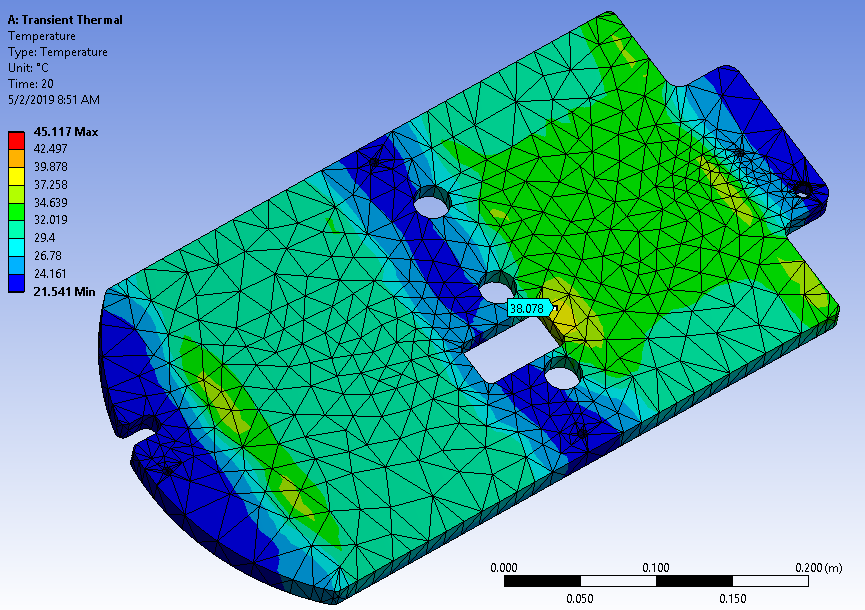
\includegraphics[width=0.8\textwidth]{final/fig/Top_Plate_3.png}
    \caption{Thermal Profile of Top Plate Base}
    \label{fig:Top_Plate_3}
\end{figure}

\begin{figure}[!htb]
    \centering
    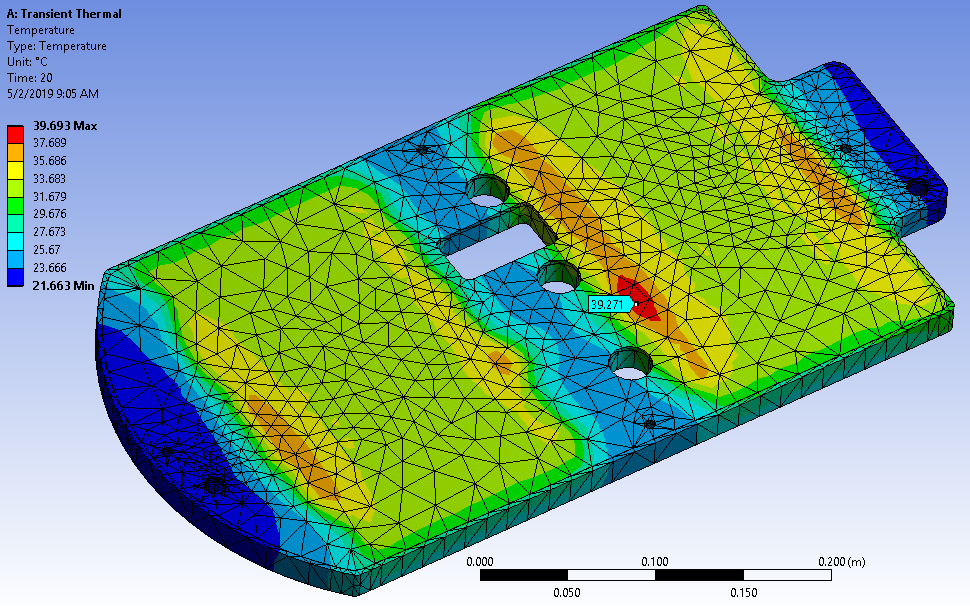
\includegraphics[width=0.8\textwidth]{final/fig/Middle_Plate_1.png}
    \caption{Thermal Profile of Middle Plate Cover}
    \label{fig:Middle_Plate_1}
\end{figure}


The thermal profile of the cover of the middle plate as shown in Figure \ref{fig:Middle_Plate_1} shows a maximum temperature of $40\degree\unit{C}$. The maximum temperatures seen in the fins and the bottom side of the middle plate are $35\degree\unit{C}$ and $27\degree\unit{C}$ as shown in the thermal profiles in  Figure \ref{fig:Middle_Plate_2} and Figure \ref{fig:Middle_Plate_3} respectively. The thermal profiles of the bottom of the top plate and the top of the middle plate are similar in the analysis as they both see similar heat fluxes. The finite element analysis validates the design and shows that the cooling plates can dissipate the heat generated by the batteries while keeping them under the SapceX requirement of $50\degree\unit{C}$.

\begin{figure}[!htb]
    \centering
    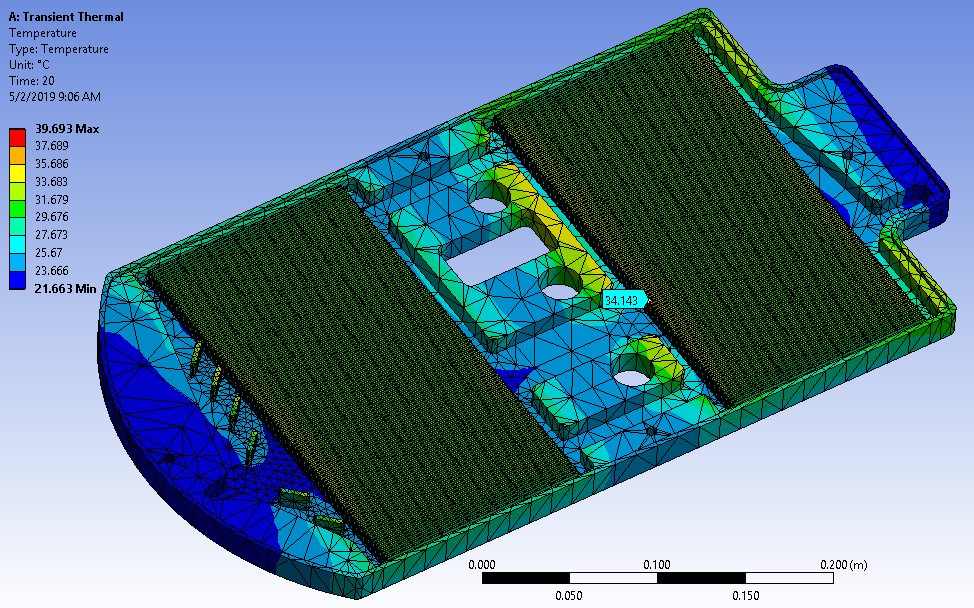
\includegraphics[width=0.8\textwidth]{final/fig/Middle_Plate_2.png}
    \caption{Thermal Profile of Middle Plate Fins}
    \label{fig:Middle_Plate_2}
\end{figure}

\begin{figure}[!h]
    \centering
    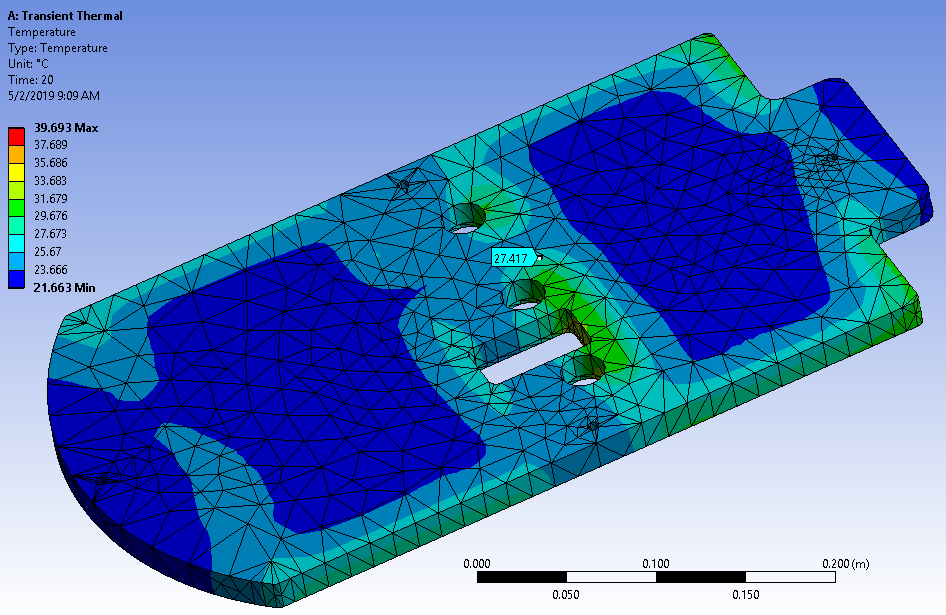
\includegraphics[width=0.8\textwidth]{final/fig/Middle_Plate_3.png}
    \caption{Thermal Profile of Middle Plate Base}
    \label{fig:Middle_Plate_3}
\end{figure}

%========================================================================
\section{Demonstration}
Novark Technologies generously agreed to ship a spare set of fins which the team utilised to manufacture a full-size replica of the thermal plate for demonstration purposes. This replica is made up of acrylic plates and the fins. The model is nonfunctional because it cannot be filled with water, but it is a useful visual aid. This demonstration piece can be seen in Figure \ref{fig:demo1} with a cross sectional view of the fins in Figure \ref{fig:demo2}.

\begin{figure}[!htb]
    \centering
    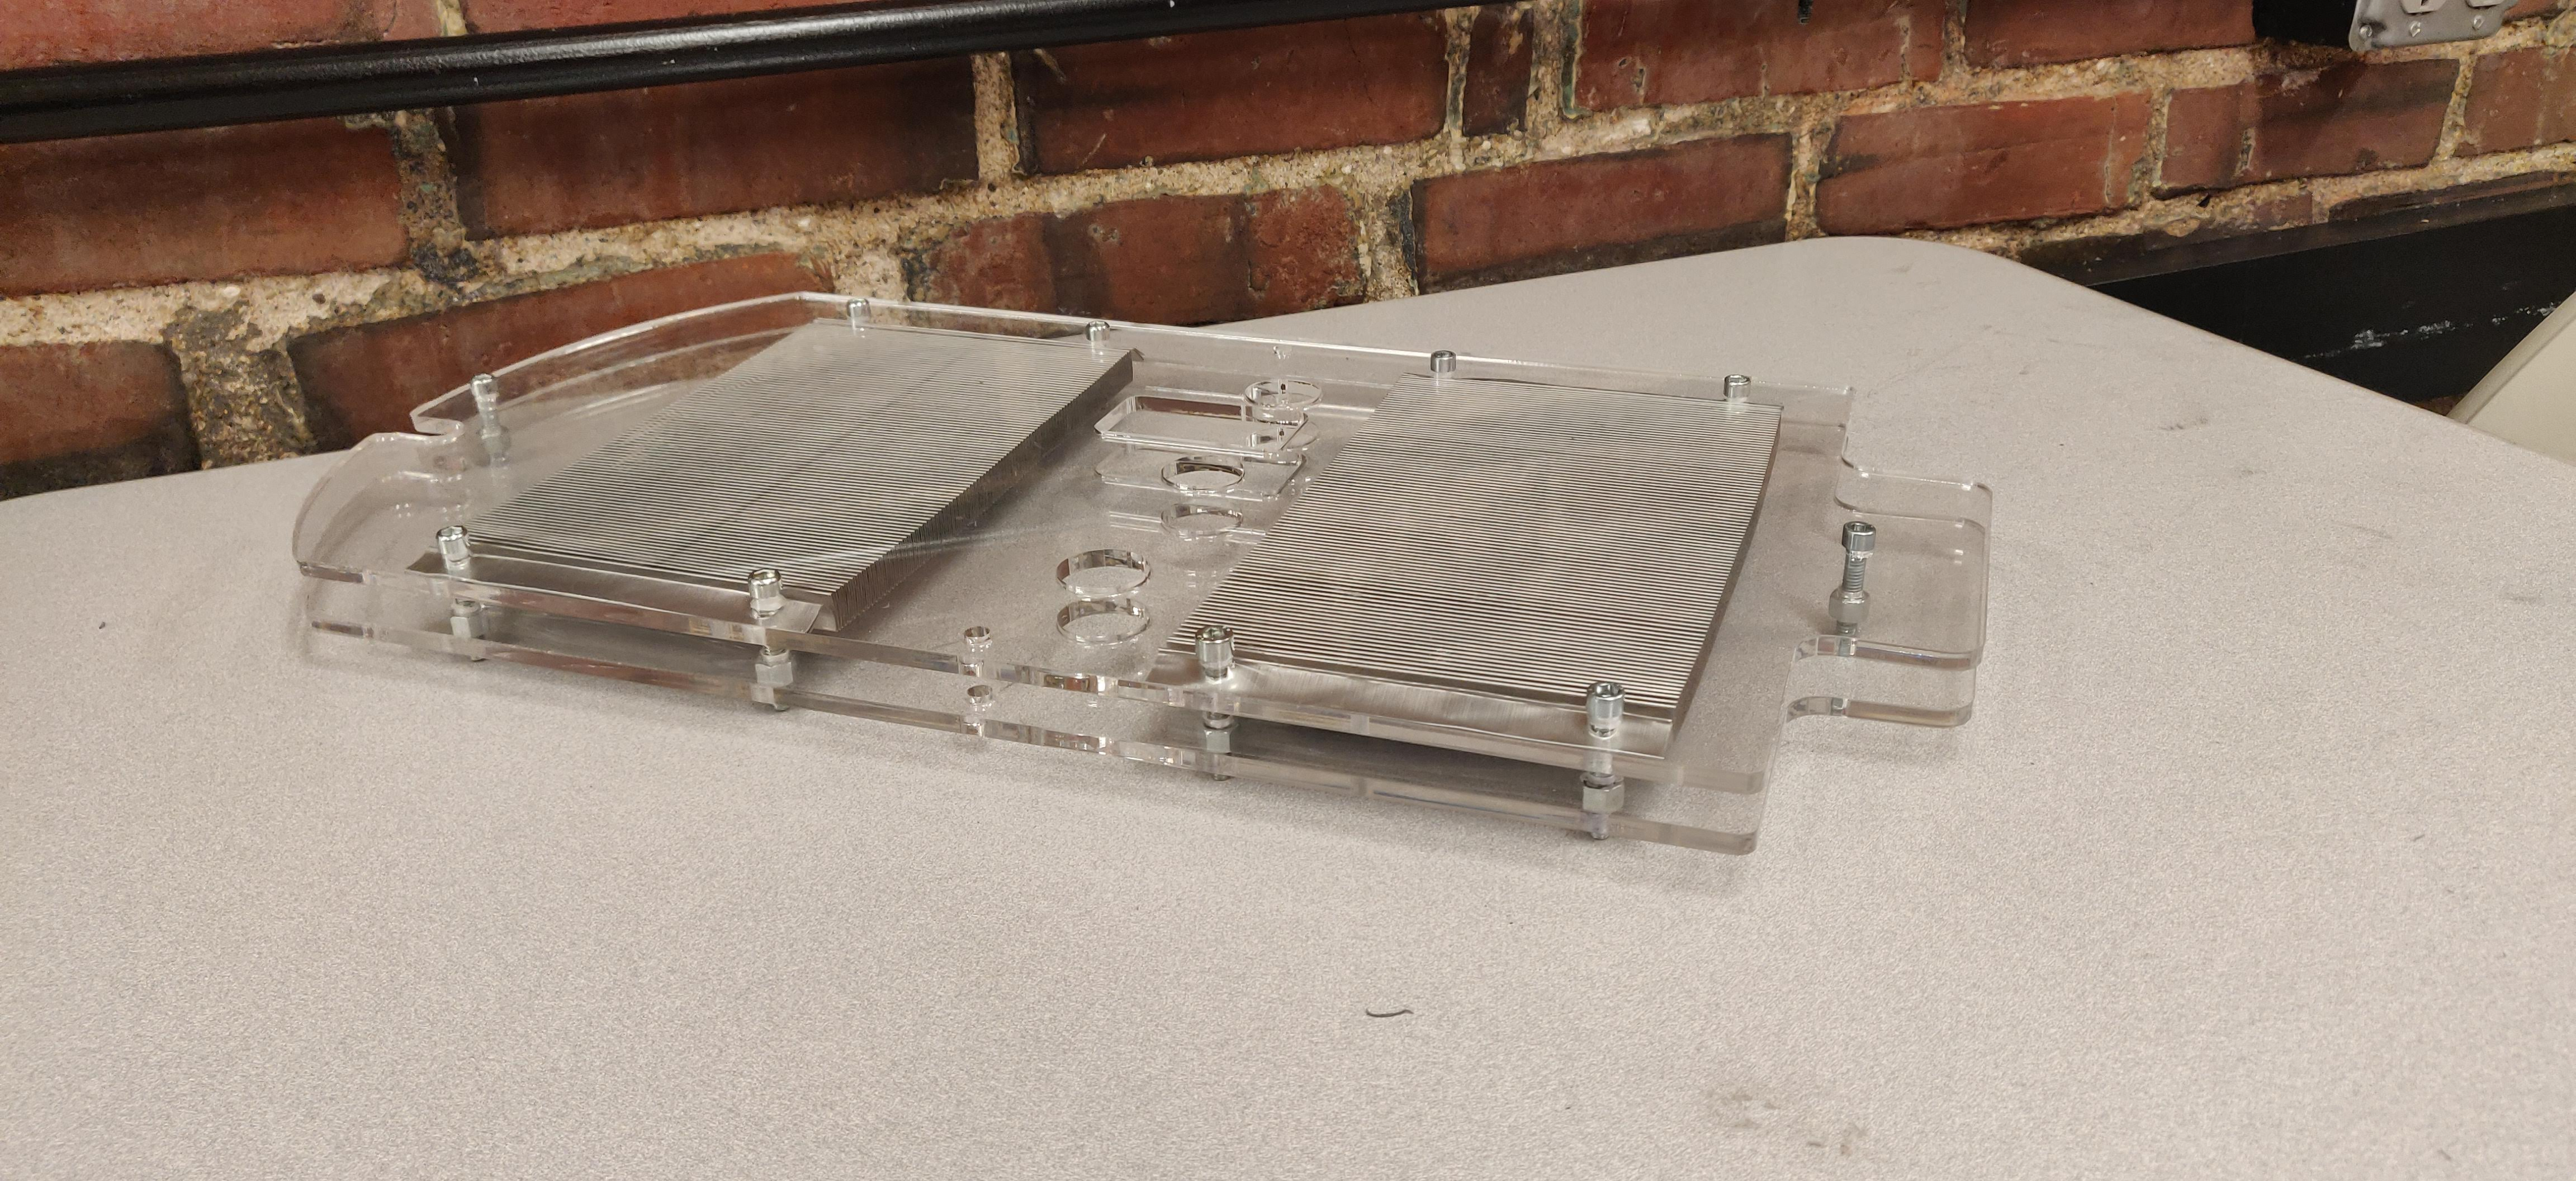
\includegraphics[width=0.8\textwidth]{final/fig/demo.jpg}
    \caption{Demonstration Replica}
    \label{fig:demo1}
\end{figure}

\begin{figure}[!htb]
    \centering
    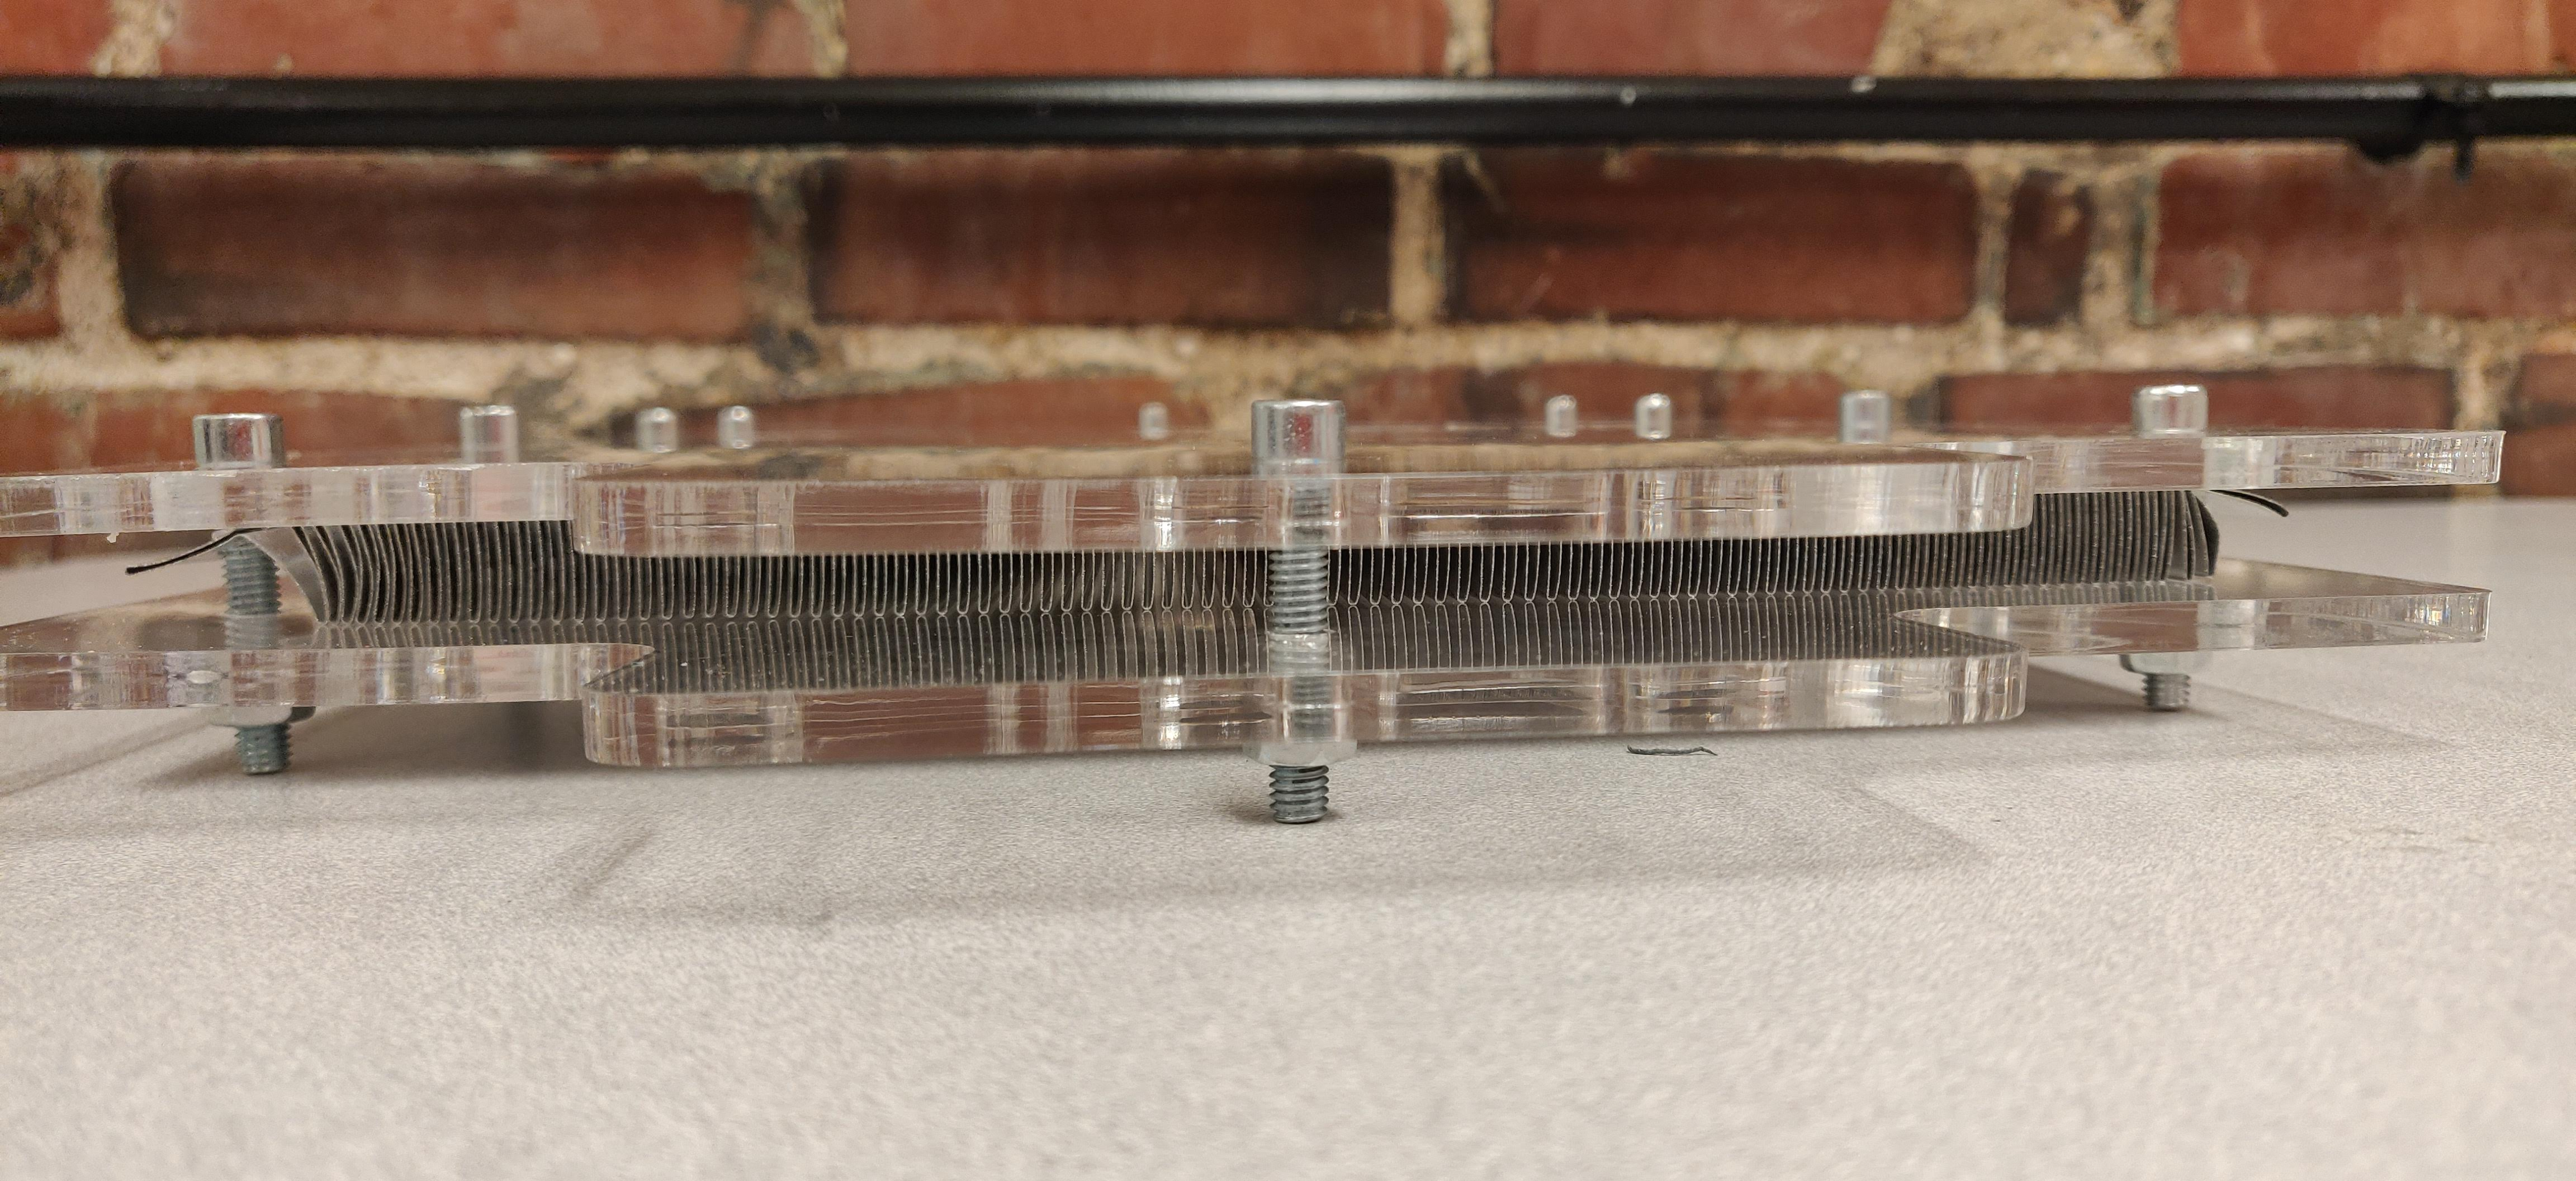
\includegraphics[width=0.8\textwidth]{final/fig/demo_cross.jpg}
    \caption{Demonstration Fins}
    \label{fig:demo2}
\end{figure}

%========================================================================
\section{Budget}\label{section:budget}
The greatest cost incurred by the team is in purchasing a single Li-Po battery module for testing. The project sponsor, Novark Technologies, generously agreed to manufacture the cooling plates in house at no charge to the team. The shipping and customs fee was paid for by the senior design team. Remaining costs incurred were for testing supplies. Equipment such as a high-power resistor and an a thermal camera were loaned from the University of Illinois Department of Mechanical Science and Engineering (MechSE). All shipping was handled by the MechSE Business Office. The total cost incurred to the team was $\$1,208$. The overall cost of the project is $\$3,208$.

\begin{table}[!htb]
  \centering
    \caption{Updated Project Budget}
    \label{table:budget}
	\begin{tabular}{r | r | c | c c}
	& \multirow{2}{*}{\textbf{Item}} & \textbf{Unit Price} & \textbf{Quantity} & \textbf{Total} \\
	&                                & \textbf{\$/Unit}    & \textbf{Unit}     & \textbf{\$}
	 \\ \hline
		
	
    \multirow{1}{*}{Cost to Novark}  & Cold Plate Manufacturing           & 2      &1000    & 2000  \\  
    \hline
    \multirow{9}{*}{Cost to Team}    & Li-Po 6S4P $22.2\unit{V}$ Battery  & 540   & 1   & 540 \\
	                                 & Battery Connectors                 & 7.50  & 4   & 30  \\ 
	                                 & Resistor Connectors                & 6     & 2   & 12  \\ 
	                                 & $4\unit{AWG}$ Wire                 & 35    & 1   & 35  \\
	                                 & Cooling Plate Shipping             & 365   &1    &365  \\  
	                                 & Customs Fee                        & 175   &1    &175  \\ 
	                                 & Fuse                               & 11    &1    &11  \\
	                                 & Acrylic Sheets                     & 20    &2    &40  \\
	\hline
	
	& & & \textbf{Total Cost to Team} & \textbf{\$1208} \\
	\end{tabular}
\end{table}

%========================================================================
\section{Recommendations}
\subsection{Water-Bath Test}
Quantifying the relationship between battery internal resistance and operating temperature improve the estimates on heat generation obtained in Section \ref{prop}. The battery is to be immersed in a water bath held at known temperatures in the $15$--$45\degree\unit{C}$ range while being discharged as shown in Fig.~\ref{fig:Water-Bath Test}. The obtained correlation would be added to the theoretical model in Section \ref{prop} to obtain an improved estimate of total heat generated, that would more accurately dictate the volume of coolant required.

\begin{figure}[!h]
    \centering
    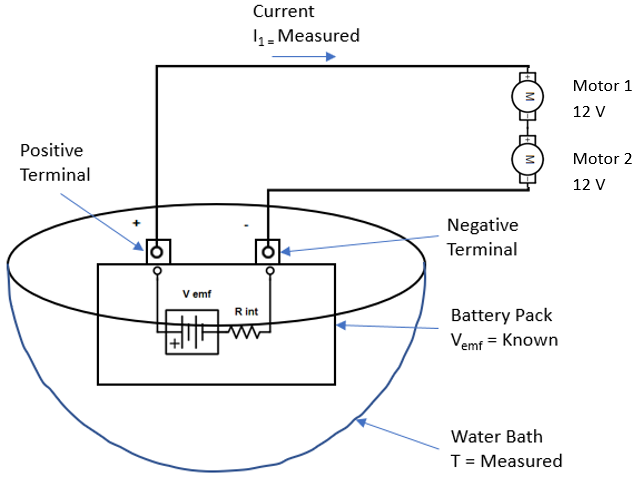
\includegraphics[width=0.7\textwidth]{final/fig/Test_Schematic.png}
    \caption{Water-Bath Test}
    \label{fig:Water-Bath Test}
\end{figure}

\subsection{Additional Cooling Plate}\label{reco-plate}
The calculations performed show that the isolated top battery will remain within the desired temperature range; however, as only one of its faces will be cooled, the battery is more prone to failure than others. The disparity can be resolved by adding a smaller cooling plate above Battery 5 in \ref{fig:batteries and plates}. The additional plate may be integrated into the rest of the system via similar piping or might even be left unconnected. In order to secure this plate within the battery box, thermal tape could be used to hold both the plate and the battery on top of the current top plate. The senior design team was unable to add a third plate due to space and weight constraints the battery box was subjected to by the hyperloop pod chassis.

\subsection{Dry Ice}
Packets of dry ice may be added to the battery box to keep the system's initial temperature below the ambient temperature before the start of the run. Sublimation of dry ice absorbs heat energy from the battery box. The battery box is fitted with a pressure relief valve so any excess pressure is released innocuously. The dry ice must not come in contact with the batteries so their temperature does not fall below the optimal range of operation. In order to decrease the temperature of the system by an additional $5\degree\unit{C}$ from the initial steady state result of $20.5\degree\unit{C}$, 0.22\unit{kg} of dry ice should be used. This calculation is shown in \ref{ice-mass}. 


%========================================================================
\section{Synopsis}
The goal of the project is to design and manufacture a compact, lightweight, effective, and reusable battery cooling solution for Illini Hyperloop. After reviewing literature, modelling power requirements, performing qualitative tests, and addressing relevant design considerations, a passive liquid cooling solution was delivered to Midwest Hyperloop. The delivered cooling solution was verified through finite element analysis to  will remove the required amount of heat from the batteries while remaining within the design constraints given. 

Unfortunately, the final prototype did not arrive in time for testing to be performed on it, but the finite element analysis performed on the plates shows that the cold plates are a sufficient solution to the problem statement. The system may be improved by supplemental future projects and its expected performance can be more accurately modelled by additional heat generation testing. The team has offered recommendations for future investigations.

The project was completed within the budget constraints and will be delivered to Illini Hyperloop on time. The cooling solution will be implemented into the hyperloop pod and will serve an important role in the performance of the propulsion system.
%========================================================================
\section{Sample Calculations}

\subsection{Coolant Volume}\label{coolant_vol}

Energy = m_{water}\cdot c_{water}\cdot \Delta T_{water}\

m_{water}=\dfrac{Energy}{c_{water}\cdot \Delta T_{water}}= 1.44 kg

V_{water}=\dfrac{m_{water}}{\rho_{water}}=1.44 L




\subsection{Steady State Initial Temperature}\label{initial_tem}

N_{batt}=5 %number of batteries

m_{batt}=N_{batt}\cdot 2.27 kg  % measure battery weight

c_{batt}=1.00 \dfrac {kJ}{kg\cdot K}

T_{batt}=30+273 K %Kelvin

m_{plates}=3.28+3.26 kg

c_{plates}=0.90 \dfrac {kJ}{kg\cdot K}

T_{plates}=30+273 K

m_{water}=997\cdot 0.0019 kg

c_{water}=4.18 \dfrac {kJ}{kg\cdot K}

T_{water}=0+273 K %Kelvin

%final temp before run
T_{final_K}=\dfrac{m_{batt}\cdot c_{batt}\cdot T_{batt}+m_{plates}\cdot c_{plates}\cdot T_{plates}+m_{water}\cdot c_{water}\cdot T_{water}}{m_{batt}\cdot c_{batt}+m_{plates}\cdot c_{plates}+m_{water}\cdot c_{water}}

T_{final_C}=T_{final_K}-273 = $20.5\degree\unit{C}$%final temp before run in degress C


Energy=302 kJ %kJ of energy to dissapate

\Delta T_{batt}=\dfrac{Energy}{m_{batt}\cdot c_{batt}} = $26\degree\unit{C}$%Temp difference
%Battery temp after run assuming that temp is constant throughout battery

T_{batt, final}=T_{final_C}+\Delta T_{batt}= $46.5\degree\unit{C}$

\subsection{Dry Ice Mass}\label{ice-mass}

N_{batt}=5 %number of batteries

m_{batt}=N_{batt}\cdot 2.27 kg  % measure battery weight

c_{batt}=1 \dfrac {kJ}{kg\cdot K}

m_{plates}=3.28+3.26 kg

c_{plates}=0.9 \dfrac {kJ}{kg\cdot K}

m_{water}=997\cdot 0.0019 kg

c_{water}=4.18 \dfrac {kJ}{kg\cdot K}

\Delta T_{combined}=$5\degree\unit{C}$

\Delta H_{sublimation}=571 \dfrac {kJ}{kg}

Q_{combined}=({m_{batt}\cdot c_{batt}+m_{plates}\cdot c_{plates}+m_{water}\cdot c_{water})\Delta T_{combined}

Q_{combined}=126 kJ

m_{dry}_{ }_{ice}=\dfrac  {Q_{combined}}{\Delta H_{dry}_{ }_{ice}}

m_{dry}_{ }_{ice}=0.22 kg


\subsection{Fin Parameters}\label{fin-area}

Energy=302 kJ

N_{batt}=5 %number of batteries

time=20 sec

U=500 W/(m^2K) % for Al water interface (approximated from eng. toolbox)

\Delta T=20 \degree K %delta K

\.{Q}=\dfrac {Energy\cdot 1000}{time \cdot N_{batt}}  W %(average power to plate section)


SA_{needed}=\dfrac{\.{Q}}{U\cdot \Delta T} m^2 % required


W=130 mm

H=12 mm

t=0.15 mm

P=2.5 mm

L=253.75 mm

N=L/P % number of fins

Perimeter=4(H-t)+2(P-2\cdot t) mm

SA_{fins}=N\cdot Perimeter\cdot W/1000000 m^2 % obtained

\.{Q}= 3000 W, SA_{needed}=0.30 m^2

\.{Q}= 6000 W, SA_{needed}=0.60 m^2

SA_{fins}=0.6835 m^2


\pagebreak
%========================================================================
\addcontentsline{toc}{section}{References}
%\bibliographystyle{IEEEtrans}
\bibliographystyle{ieeetr}

\bibliography{final} 


\end{document}